\documentclass[onecolumn, draftclsnofoot,10pt, compsoc]{IEEEtran}
\usepackage{graphicx}
\usepackage{url}
\usepackage{setspace}
\usepackage{abstract}
\usepackage{geometry}
\usepackage{listings}
\usepackage{color}
\geometry{textheight=9.5in, textwidth=7in}
\parindent = 0.0 in
\parskip = 0.1 in

% set up code syntax highlighting
\definecolor{coolblack}{rgb}{0.0, 0.18, 0.39}
\definecolor{darkgreen}{rgb}{0.0, 0.5, 0.0}
\definecolor{orange}{rgb}{0.8, 0.33, 0.0}
\lstdefinestyle{customc}{
  belowcaptionskip=1\baselineskip,
  breaklines=true,
  frame=L,
  xleftmargin=\parindent,
  language=C++,
  showstringspaces=false,
  basicstyle=\footnotesize\ttfamily,
  keywordstyle=\bfseries\color{blue},
  commentstyle=\itshape\color{darkgreen},
  identifierstyle=\color{coolblack},
  stringstyle=\color{orange},
}

\lstdefinestyle{customasm}{
  belowcaptionskip=1\baselineskip,
  frame=L,
  xleftmargin=\parindent,
  language=[x86masm]Assembler,
  basicstyle=\footnotesize\ttfamily,
  commentstyle=\itshape\color{purple!40!black},
}

\lstset{style=customc}
% end syntax highlighting setup

% 1. Fill in these details
\def \CapstoneTeamName{WebXR Team}
\def \CapstoneTeamNumber{47}
\def \GroupMemberOne{Brooks Mikkelsen}
\def \GroupMemberTwo{Evan Brass}
\def \GroupMemberThree{Jonathan Jones}
\def \GroupMemberFour{Brandon Mei}
\def \GroupMemberFive{Tim Forsyth}
\def \CapstoneProjectName{WebXR Physics Simulation}
\def \CapstoneSponsorCompany{Intel}
\def \CapstoneSponsorPerson{Alexis Menard}

% 2. Uncomment the appropriate line below so that the document type works
\def \DocType{	%Problem Statement
				%Requirements Document
				%Technology Review
				%Design Document
				Winter Progress Report
				}
			
\newcommand{\NameSigPair}[1]{\par
\makebox[2.75in][r]{#1} \hfil 	\makebox[3.25in]{\makebox[2.25in]{\hrulefill} \hfill		\makebox[.75in]{\hrulefill}}
\par\vspace{-12pt} \textit{\tiny\noindent
\makebox[2.75in]{} \hfil		\makebox[3.25in]{\makebox[2.25in][r]{Signature} \hfill	\makebox[.75in][r]{Date}}}}
% 3. If the document is not to be signed, uncomment the RENEWcommand below
%\renewcommand{\NameSigPair}[1]{#1}

%%%%%%%%%%%%%%%%%%%%%%%%%%%%%%%%%%%%%%%
\begin{document}
\begin{titlepage}
    \pagenumbering{gobble}
    \begin{singlespace}
    	%\includegraphics[height=4cm]{coe_v_spot1}
        \hfill 
        % 4. If you have a logo, use this includegraphics command to put it on the coversheet.
        %\includegraphics[height=4cm]{CompanyLogo}   
        \par\vspace{.2in}
        \centering
        \scshape{
            \huge CS Capstone \DocType \par
            {\large\today}\par
            \vspace{.5in}
            \textbf{\Huge\CapstoneProjectName}\par
            \vfill
            {\large Prepared for}\par
            \Huge \CapstoneSponsorCompany\par
            \vspace{5pt}
            {\Large\NameSigPair{\CapstoneSponsorPerson}\par}
            {\large Prepared by }\par
            Group \CapstoneTeamNumber\par
            % 5. comment out the line below this one if you do not wish to name your team
            %\CapstoneTeamName\par 
            \vspace{5pt}
            {\Large
                \NameSigPair{\GroupMemberOne}\par
                \NameSigPair{\GroupMemberTwo}\par
                \NameSigPair{\GroupMemberThree}\par
                \NameSigPair{\GroupMemberFour}\par
                \NameSigPair{\GroupMemberFive}\par
            }
            \vspace{20pt}
        }
        %\renewcommand{\abstracttextfont}{\sffamily}
        \begin{abstract}
        % 6. Fill in your abstract    
        	The WebXR Device API provides the interfaces necessary to enable developers to build a powerful, frictionless, and more features across a wide variety of hardware form factors. Our virtual reality physics simulation showcase the uses of WebXR Device API. This document is a progress report that is intended to outline our project purposes and goals, progress so far, discusses the work completed and challenges encountered during Winter Term. This report shows our progress of a beta level functionality as of Winter Term 2019.
        \end{abstract}     
    \end{singlespace}
\end{titlepage}
\newpage
\pagenumbering{arabic}
\tableofcontents
% 7. uncomment this (if applicable). Consider adding a page break.
%\listoffigures
%\listoftables

\clearpage

% 8. now you write!
\section{Project Purposes and Goals}
Our project is a virtual reality physics simulation that can run entirely on the web. The project is intended to show off the functionality of the new WebXR API. This is an API spec that is still being developed and implemented into Chrome and other browsers, so it is very dynamic for the time being. The project will provide a good example of a real application built using the WebXR API, so that future developers wishing to use the API will have something to go off of. 

Another goal of the project is to provide a simple tool for high school physics students to study the physics interactions first hand without the need for expensive lab equipment. The goal was to make our app as accessible as possible. It can run on most smartphones with an up to date version of Chrome.

\section{What we have done}
As a team, we have been busy working on beta level functionality. This functionality includes magic window, which allows mobile users to look around in the experience when they move their device. It also includes two-eye rendering, which renders the scene twice, once for each eye when the user is wearing a virtual reality headset. This beta functionality also includes a simple version of some of our physics simulations as well.  

\subsection{Brooks}
This term, I worked on getting our environment set up, including the project structure, our build tools, continuous integration, and automated deployments. For the project structure, I created a Node.js package so we could download dependencies such as Three.js from npm, the Node package manager. 

I also set up the asset bundler, so that we could have it watch for changes as we are developing, and then rebuild the project and reload the page as necessary. This also allowed us to use modules to improve the readability of our code, while still being able to run in browsers that do not support JavaScript module syntax. 

I set up our GitHub repo to automatically notify continuous integration whenever we made a push to a branch or pull request so that it would rebuild our project on the Circle CI's continuous integration server. I added linting to it to help maintain high quality code and find errors in syntax. Also, for each push, I set up automatic deployments so that it would build and serve that version of the site. This way we can send each other (and other people such as our client) links to specific versions of the site. 

Since that only took up a few weeks at the beginning, I then went on to help define the core structure of the code. I proposed a class for each experience, each of which inherit from a parent class with standard functionalities such as an animation function and a state object. I refactored our project to adapt to this structure after discussing it with our client my fellow team members. This included migrating the site to a single page application format, with a different route for each physics simulation.

I also built an asset loading system that allows the developer of each scene to specify all the assets required, and then goes to fetch said assets. Once the assets are all completely loaded, a callback function is raised, so that they can be added into the scene and the scene will start rendering. I also built a loading screen that would automatically display while everything is loading. 

The last thing I did was to build out an beta functionality of the planets demo. This included realistic physics for orbiting planets (using Newton's law of universal gravitation). The following code updates the position of a planet as another planet acts upon it. 
\begin{lstlisting}
export const G = 6.673e-11;

/**
 * returns force of gravity on p1 and p2 from the other
 *
 * @param {Vector3} p1
 * @param {Vector3} p2
 */
function forceGrav(p1, p2, m1, m2) {
  const rSquared = p1.distanceToSquared(p2);

  return (G * m1 * m2) / rSquared;
}

/**
 * moves planet p1 by amount other planet is acting on it
 *
 * @param {Planet} p1 planet to move
 * @param {Vector3} pos1 old position planet to move
 * @param {Vector3} pos2 old position of other planet
 * @param {number} mass2 mass of other planet
 * @param {number} time delta time
 */
function movePlanet(p1, pos1, pos2, mass2, time) {
  const forceScalar = forceGrav(pos1, pos2, p1.mass, mass2);

  const accelerationVec = relativePos(pos1, pos2)
    .multiplyScalar(forceScalar) // force
    .divideScalar(p1.mass); // acceleration

  // update position using the following two vectors
  const d1 = new Vector3()
    .copy(p1.velocity)
    .multiplyScalar(time);

  const d2 = new Vector3()
    .copy(accelerationVec)
    .multiplyScalar(0.5 * (time ** 2));

  p1.mesh.position
    .add(d1)
    .add(d2);

  // update vel
  accelerationVec.multiplyScalar(time);
  p1.velocity.add(accelerationVec); // accelerationVec is now a*t
}
\end{lstlisting}
The `movePlanet` function is called for each pair of two planets in the system, ensuring that they all orbit in a realistic manner. 

The following is a screenshot of what the orbiting planets experience currently looks like.

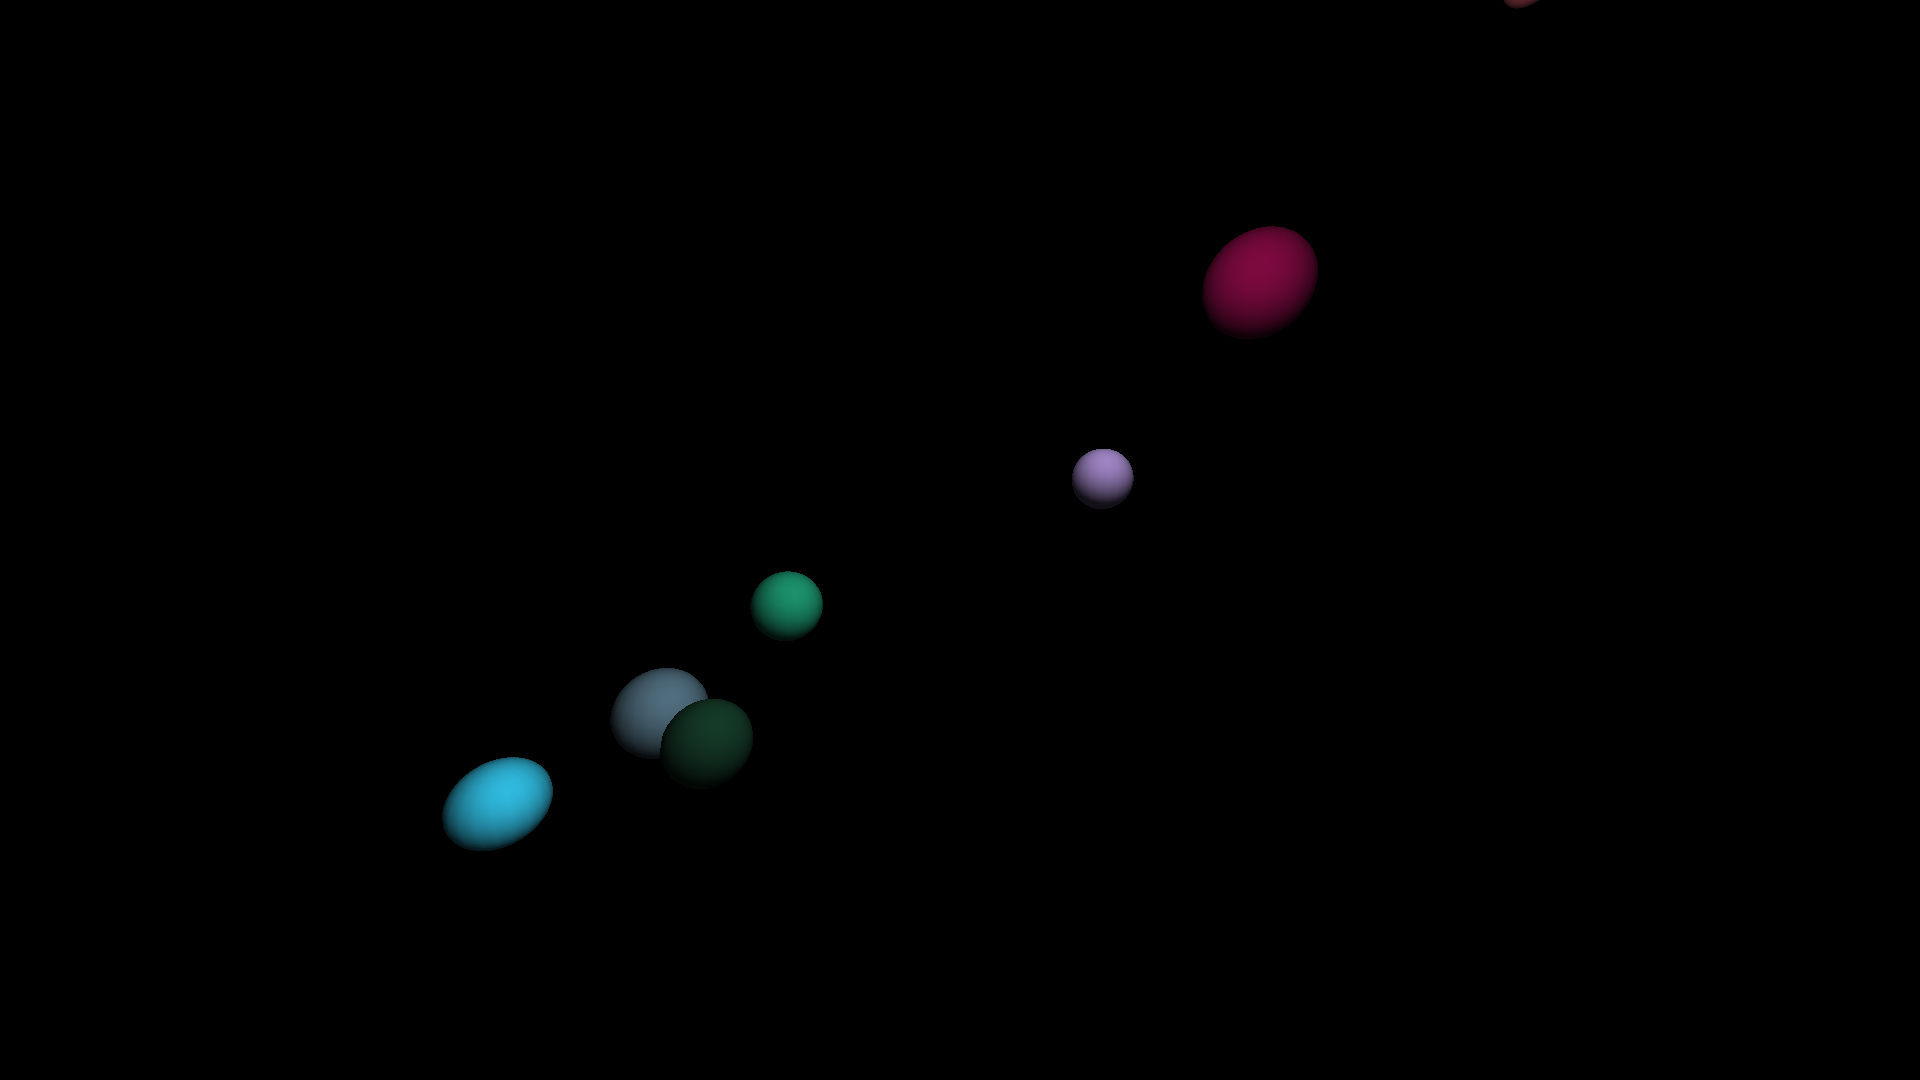
\includegraphics[width=\linewidth]{images/planets.png}

\subsection{Tim}
My work started with setting up a basic room using Three.js that could eventually be used as a home lobby connecting to the other rooms containing the experiences. Afterwards, I began working on user input to let the user move throughout the scenes. 

\subsubsection{Progress}
First, I created keyboard and mouse controls as that is the most accessible input scheme to use for basic testing of scenes. These controls are made using a Three.js tool called PointerLockControls which allows the user to move the camera using their mouse when the mouse pointer has been locked into the screen. For the keyboard movement, keydown and keyup event listeners are used to detect when a key has been pressed, figure out which key it is, and then perform the specific action associated with pressing that key, such as moving forward when the ‘W’ key or the up arrow is pressed. Using a Three.js 3D vector, I created a velocity vector to keep track of the x and z movement. When a key associated with movement is pressed, the correct amount of movement is applied to this velocity vector; for example, when the ‘S’ key is pressed, the “movement distance”, which is how far the user is moved each frame, is added to the z value of the velocity vector. This means, theoretically, it should be easy to produce movement in 45 degree angles when two keys are pressed with one moving in the x direction and the other in z. However, I needed some way of keeping track of when multiple keys have been pressed. This was done using a rather interesting solution making use of bitwise operations: 

\begin{lstlisting}
export function onKeyDown(event) {
 switch (event.keyCode) {
   case Key.Up:
   case Key.W:
     movingDirection |= Direction.Forward;
     break;
   case Key.Left:
   case Key.A:
     movingDirection |= Direction.Left;
     break;
   case Key.Down:
   case Key.S:
     movingDirection |= Direction.Backward;
     break;
   case Key.Right:
   case Key.D:
     movingDirection |= Direction.Right;
     break;
   default:
     break;
 }
}
\end{lstlisting}

This is called when the keydown event listener is fired. The movingDirection variable is simply an integer while Direction is a constant object exported from the control-utils file with the values used for detecting the correct movement:

\begin{lstlisting}
export const Direction = {
 Stopped: 0,
 Left: 1,
 Right: 2,
 Forward: 4,
 Backward: 8
};
\end{lstlisting}

These numbers are specifically chosen due to how they interact with each other when doing bitwise operations such as OR and AND. ORing these numbers will accomplish essentially the same thing as adding the values together. In the callback function for the keyup event listener, the AND and NOT operations are used:

\begin{lstlisting}
export function onKeyUp(event) {
 switch (event.keyCode) {
   case Key.Up:
   case Key.W:
     movingDirection &= ~Direction.Forward;
     break;
   case Key.Left:
   case Key.A:
     movingDirection &= ~Direction.Left;
     break;
   case Key.Down:
   case Key.S:
     movingDirection &= ~Direction.Backward;
     break;
   case Key.Right:
   case Key.D:
     movingDirection &= ~Direction.Right;
     break;
   default:
     break;
 }
}
\end{lstlisting}

This essentially does the same thing as subtracting the direction value from the total movingDirection number. In these cases, using bitwise operations is not necessary, but it is more efficient in terms of processing. When it becomes essential is when trying to figure out which keys are currently being pressed using this movingDirection number:

\begin{lstlisting}
const movingDistance = 100.0 * delta;

if ((movingDirection & Direction.Forward) === Direction.Forward) {
  velocity.z -= movingDistance;
}
if ((movingDirection & Direction.Backward) === Direction.Backward) {
  velocity.z += movingDistance;
}
if ((movingDirection & Direction.Left) === Direction.Left) {
  velocity.x -= movingDistance;
}
if ((movingDirection & Direction.Right) === Direction.Right) {
  velocity.x += movingDistance;
}
\end{lstlisting}

Due to the specific numbers that were chosen, when the movingDirection value is ANDed with the specific Direction value, it will result in that Direction value as long as it has yet to be “subtracted” away. For example, if the ‘W’ and ‘A’ key are pressed, then the movingDirection would be 4 (Direction.Forward) + 1 (Direction.Left), or 5.  5 ANDed with 4 results in 4, while 5 ANDed with 1 results in 1. However, 5 ANDed with 2 or 5 ANDed with 8 both result in 0. This works with every combination of these numbers to correctly detect which keys are currently pressed and update the position accordingly.

After the keyboard controls were implemented, I moved onto the touch controls. This was done using pointer and touch event listeners pointerdown, pointermove, and pointerup with similar event listeners touchstart, touchmove and touchend set in place to support browsers without the pointer listeners. The pointerdown callback simply stored where on the screen was touched. The pointermove callback is where the direction in which the user has moved their finger along the screen is calculated using the computeDirection method:

\begin{lstlisting}
const deltaX = ev.x - touchscreen.joystickOriginX;
const deltaY = ev.y - touchscreen.joystickOriginY;
computeDirection(deltaX, deltaY);
\end{lstlisting}

The variables deltaX and deltaY are calculated by simply finding the difference of delta of the x and y values in relation to the original touch point from the pointerdown event.

\begin{lstlisting}
export function computeDirection(deltaX, deltaY) {
  if (deltaX > 70) {
    velocity.x = -70;
  }
  if (deltaX < -70) {
    velocity.x = 70;
  }
  if (deltaY > 70) {
    velocity.z = -70;
  }
  if (deltaY < -70) {
    velocity.z = 70;
  }
  if ((deltaX <= 70 && deltaX >= -70) && (deltaY <= 70 && deltaY >= -70)) {
    joystick.style.transform = `translate(${deltaX}px,${deltaY}px)`;
    velocity.x = -deltaX;
    velocity.z = -deltaY;
  } else if ((deltaX <= 70 && deltaX >= -70) && (deltaY > 70)) {
    joystick.style.transform = `translate(${deltaX}px,70px)`;
  } else if ((deltaX <= 70 && deltaX >= -70) && (deltaY < -70)) {
    joystick.style.transform = `translate(${deltaX}px,-70px)`;
  } else if ((deltaY <= 70 && deltaY >= -70) && (deltaX > 70)) {
    joystick.style.transform = `translate(70px,${deltaY}px)`;
  } else if ((deltaY <= 70 && deltaY >= -70) && (deltaX < -70)) {
    joystick.style.transform = `translate(-70px,${deltaY}px)`;
  }
}
\end{lstlisting}

Computing the direction is as simple as using these deltaX and deltaY values as the x and z values in a velocity vector that is used to move the user. The first 4 if statements are there to set a boundary limit so that users wouldn't move insanely quick by swiping their finger a long distance across the screen quickly. The last if statement is for the general case in which the user keeps their finger within the 140 by 140 pixel range allocated for the joystick motion. Following the if statements are several else statements used for making the joystick animation much smoother when the user moves their finger past the bounded range.

To conclude my work, I added a method of opening the canvas in fullscreen mode for both keyboard and mouse as well as touch controls. On a desktop with keyboard and mouse, it will simply open in fullscreen when you click into the canvas. For mobile devices, there is a fullscreen button that launches fullscreen mode when pressed. To do this, I set up a control utils file with several utility methods that both the keyboard controls and touch controls could take from. The fullscreen code is rather straightforward using event listeners and built in dom calls such as requesting full screen and checking if it is currently active.

I also aided Jonathan with linking the two-eye immersive rendering with an Enter VR button I created, which is described in more detail in his section.

Next, I started working on the kinematic motion experience by creating spawn-able objects. I began by taking the basic Cannon.js set up from Brandon and expanded on it. So far, there are two objects: a sphere and a cube. Initially, I had done some things using a ThreeJS Raycaster to find where the user is trying to click or look at by calculating the intersection of an invisible line or ray with the objects in the scene. It would return the first object it hits and then, depending on what object it was, if you hovered over it or clicked on it, it performed a specific action, like highlighting the object or spawning a replica of the object. However, Jonathan recently implemented a nice way of dealing with object interaction using a ThreeJS Raycaster and a special object which implements ThreeJS Mesh, a TriggerMesh. I refactored my code to use the new TriggerMesh by creating the objects using a TriggerMesh instead of a ThreeJS Mesh. Then, I just had to connect the interactions I wanted to use for hovering, selecting, releasing, and exiting the object. For example, here's the code I'm using for creating the sphere that is used to spawn balls.
 
\begin{lstlisting}
    let material = new THREE.MeshPhongMaterial({ color: 'gray' });
    const ballSpawner = new TriggerMesh(this.ballGeo, material);
    ballSpawner.castShadow = true;
    ballSpawner.receiveShadow = true;
    ballSpawner.position.set(0, -1.6, -13);

    ballSpawner.addFunction('spawnBall', this._spawnBall);

    ballSpawner.hover = function () {
      if (!this.isSelected) {
        this.material.color.set(0xFF0000);
      }
    };

    ballSpawner.select = function () {
      this.functions.spawnBall();
    };

    ballSpawner.exit = function () {
      this.material.color.set(0xFFFFFF);
    };

    this.triggers.add(ballSpawner);

    const ballBody = new CANNON.Body({ mass: 0 });
    ballBody.addShape(this.ballShape);
    ballBody.position.copy(ballSpawner.position);
    this.world.addBody(ballBody);
\end{lstlisting}

The hover function highlights the sphere when hovering, the select function calls the spawnBall function, and the exit function sets the spheres color back to it's original color, white. Notice, at the end where I'm creating the CannonJS body to be associated with the TriggerMesh, I'm setting it's mass to 0. This is because in CannonJS an object with a mass of 0 will be immovable, but still interact with other objects. This means that objects will still collide with and bounce off of the spawner, but won't move it off of the table that it's set on.

In addition to spawning objects, I added some keyboard hotkeys that allow the user to manipulate physics. This includes the ability to toggle gravity off and on using 'G', reversing gravity using 'R', and toggling objects physics and animations from freezing with 'F'.

Afterwards, I implemented basic home room navigation to the other scenes using the TriggerMesh interaction on rectangles that represent doors until we can get proper 3D models. Currently, the navigation isn't optimal since the doors are only in the home scene, however, we will eventually add a door in each scene that navigates back home.

Finally, I updated a few pieces of the interface, such as changing the fullscreen button from a + to a proper fullscreen icon, moving the Enter VR to a more appropriate position in the top left corner and adding opacity to it, and adding a cross-hair to the keyboard and mouse PointerLockControls to make aiming the controls much easier.

\subsubsection{Visuals}
Using touch controls in fullscreen.

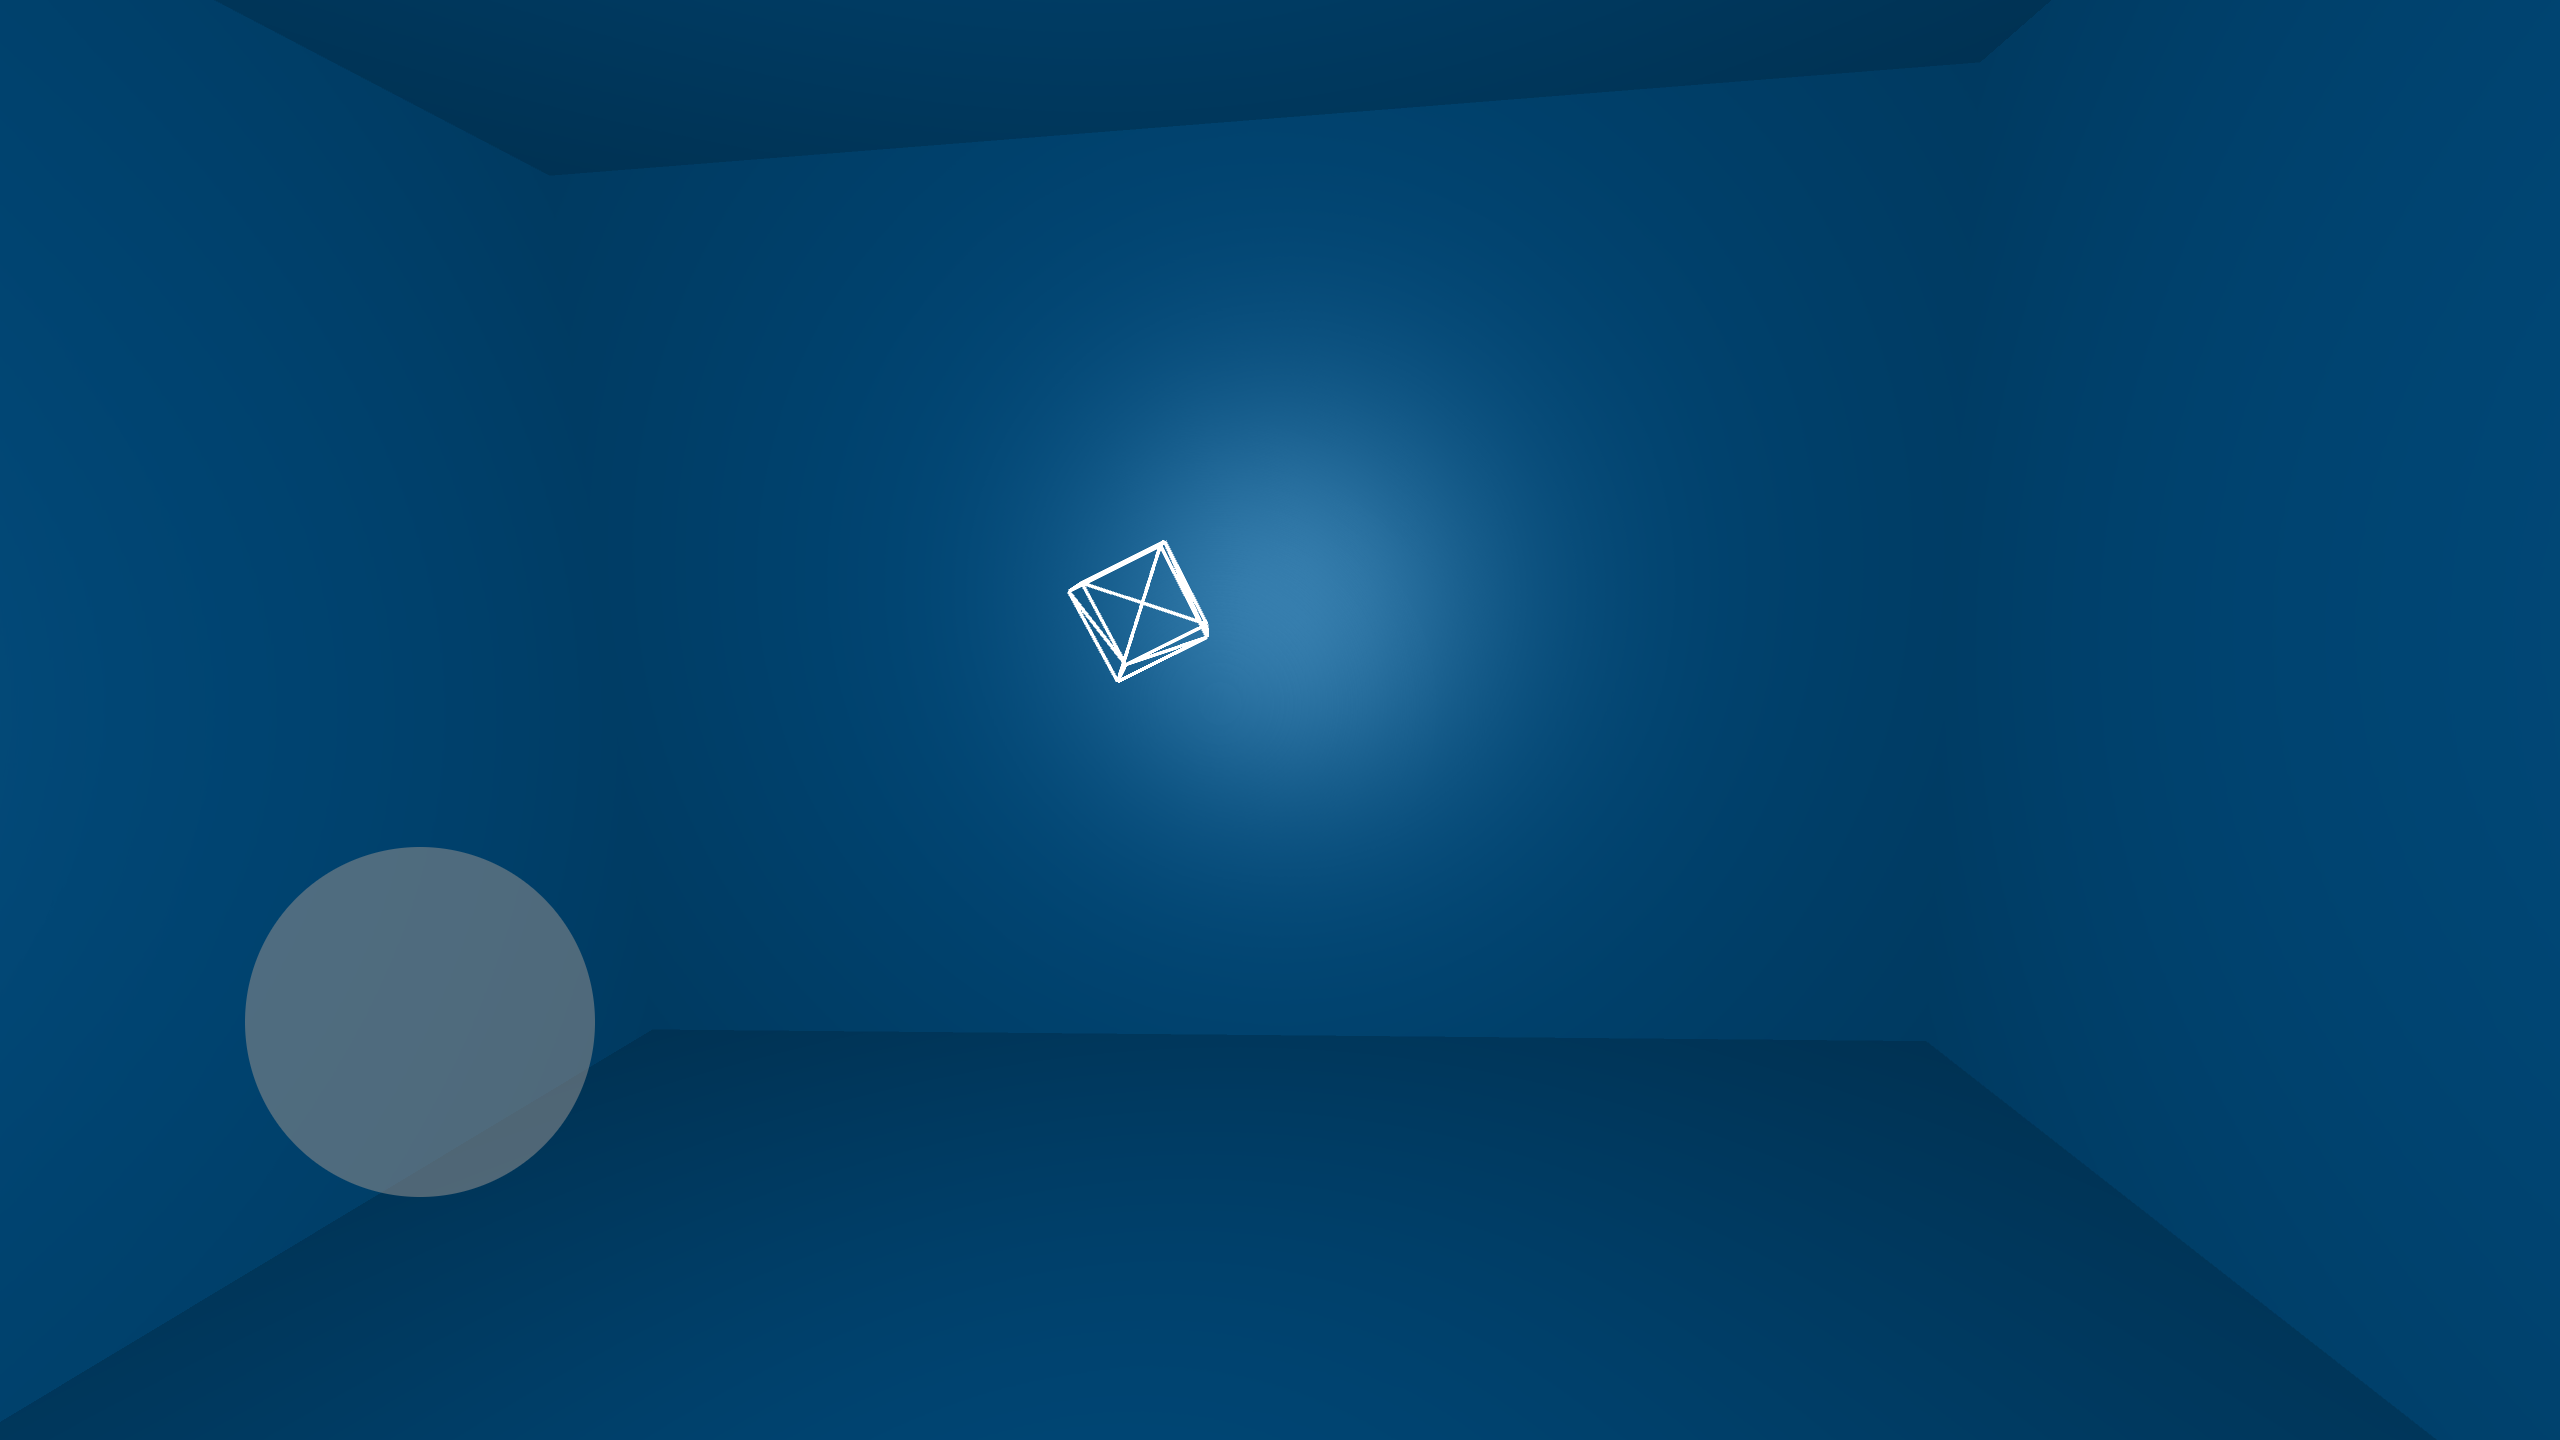
\includegraphics[width=\linewidth]{images/JoystickFullscreen.png}

\clearpage

Using touch controls in the browser window.

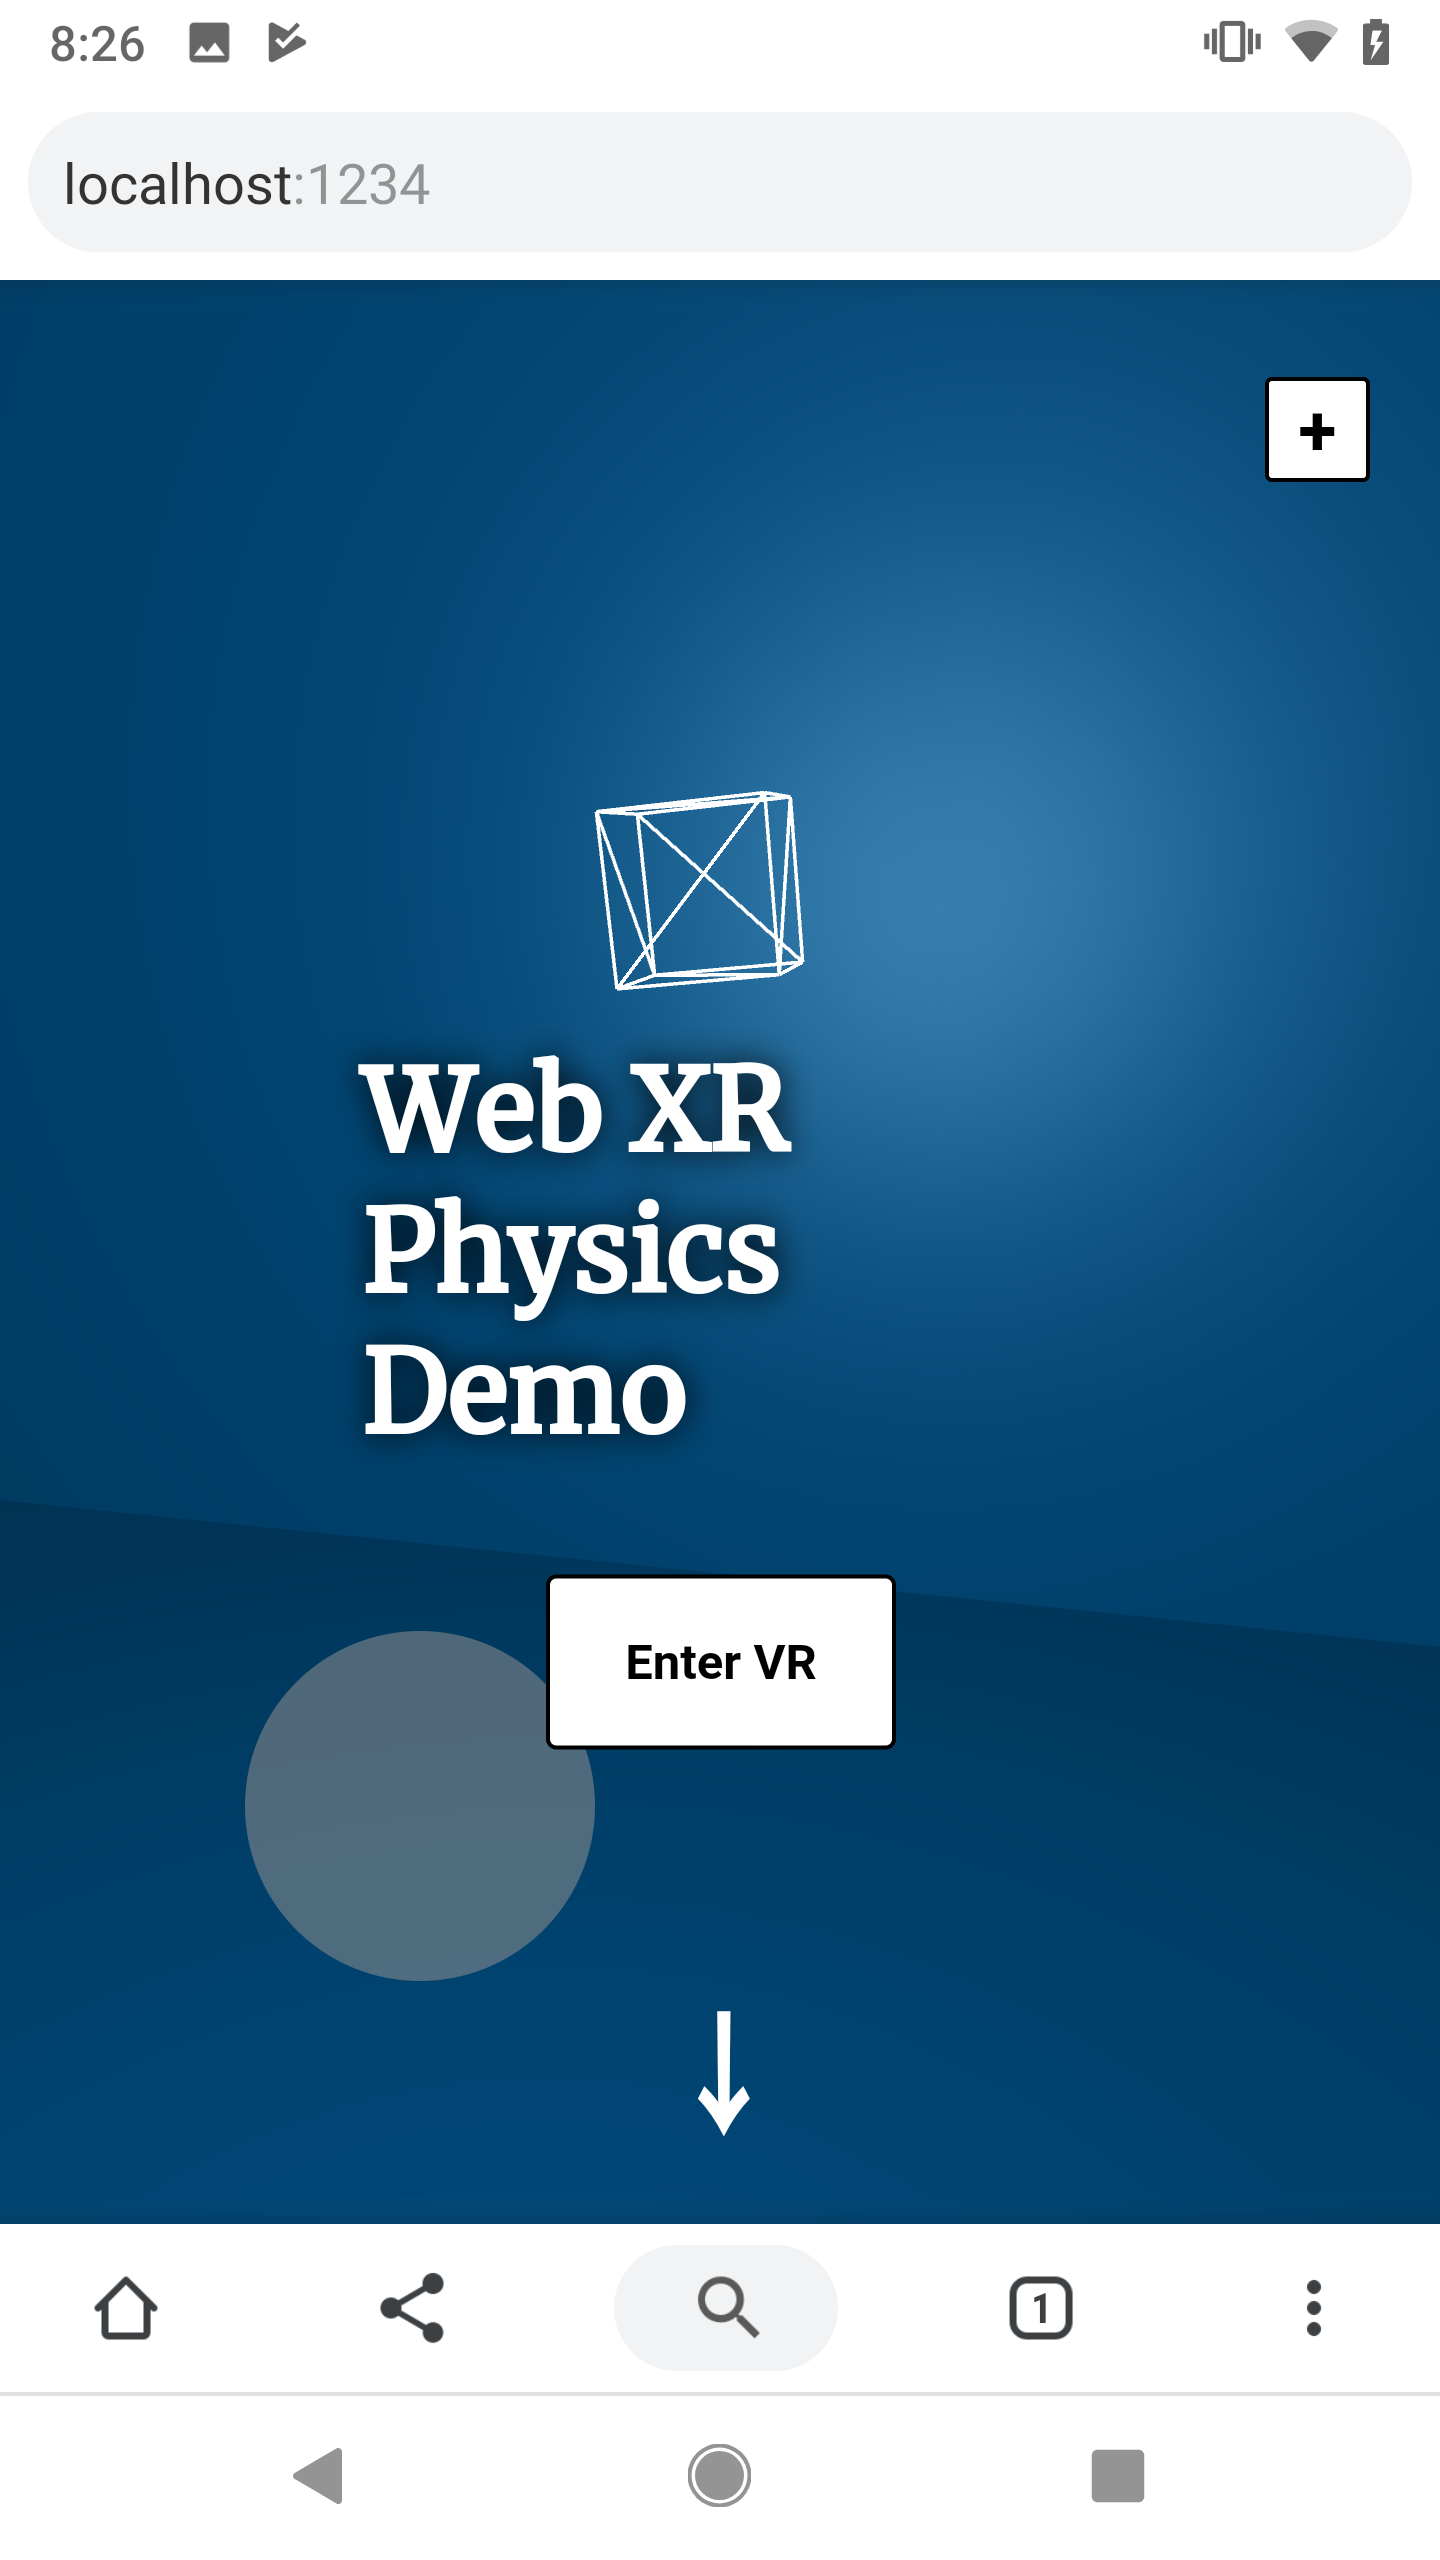
\includegraphics[width=0.35\linewidth]{images/JoystickWindow.png}

Default position of kinematic motion experience.

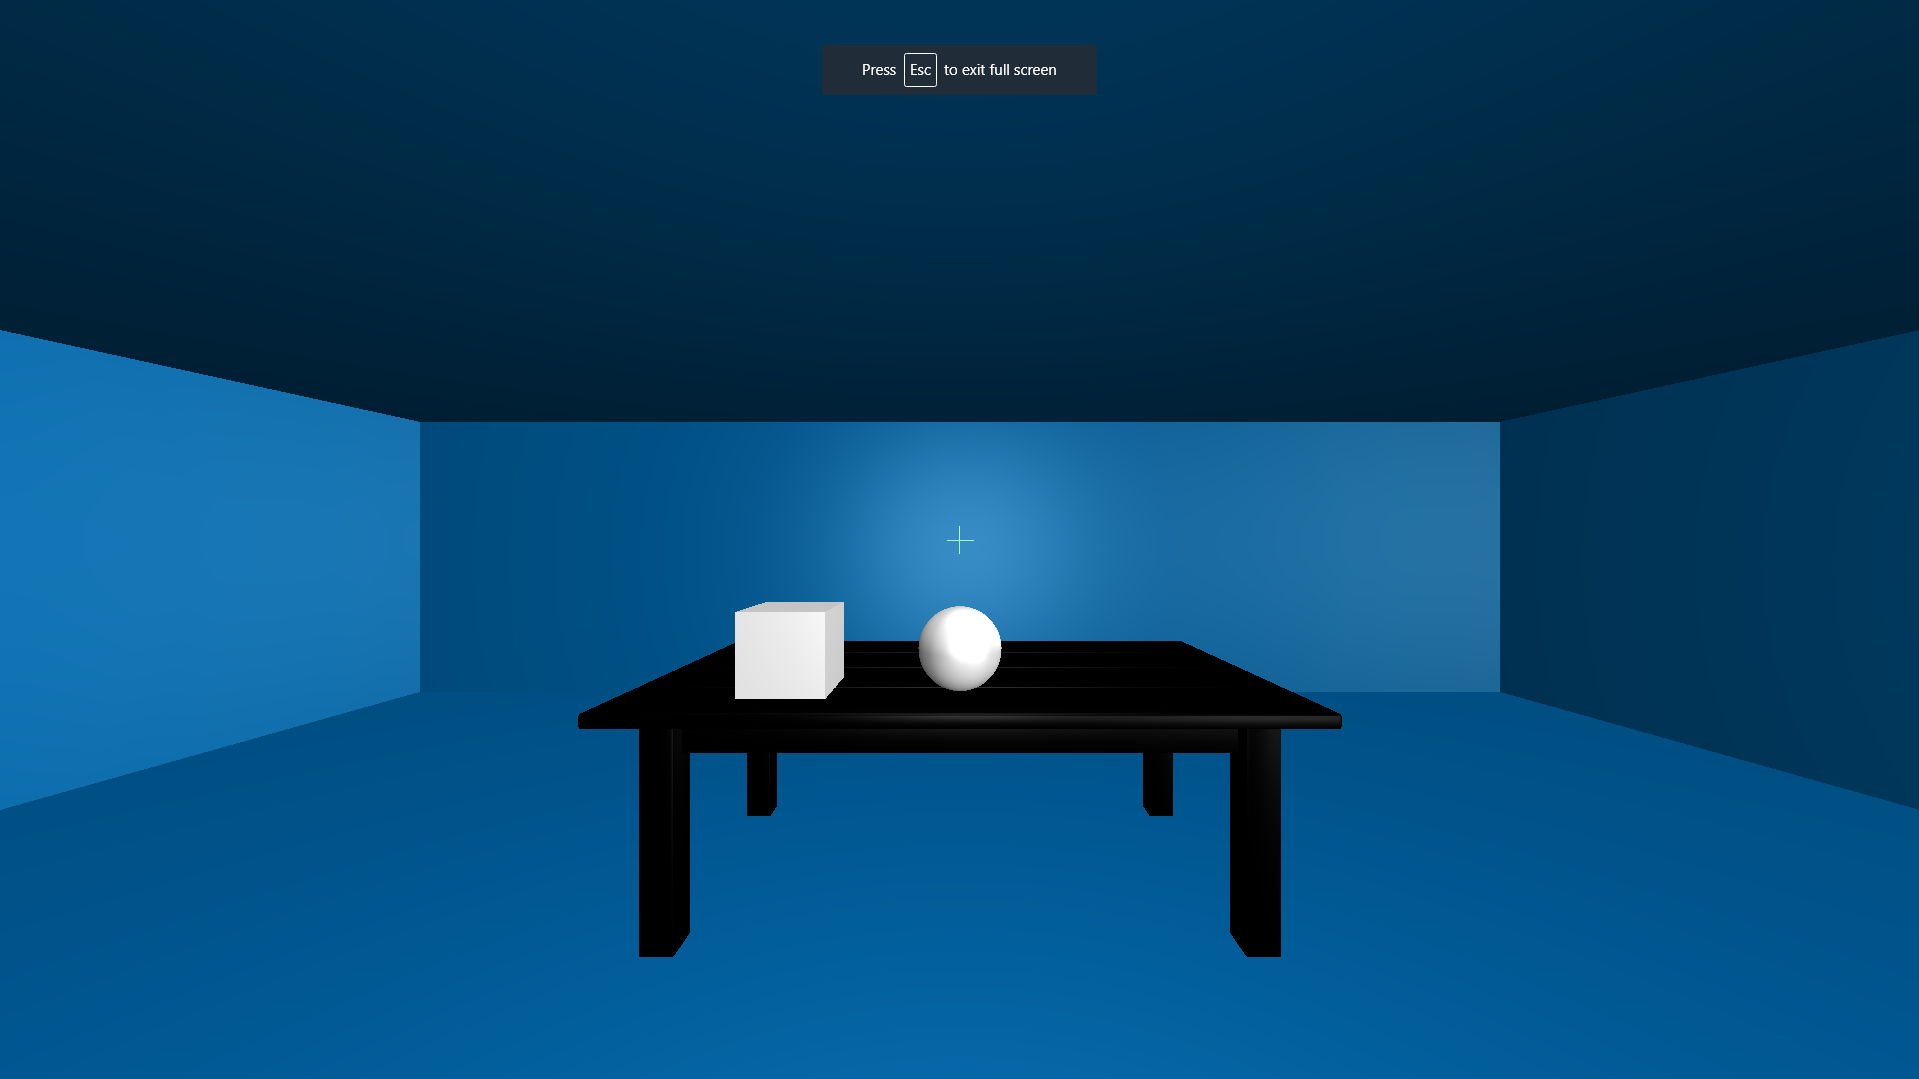
\includegraphics[width=\linewidth]{images/kinematic-default.png}

\clearpage

A bunch of objects spawned in.

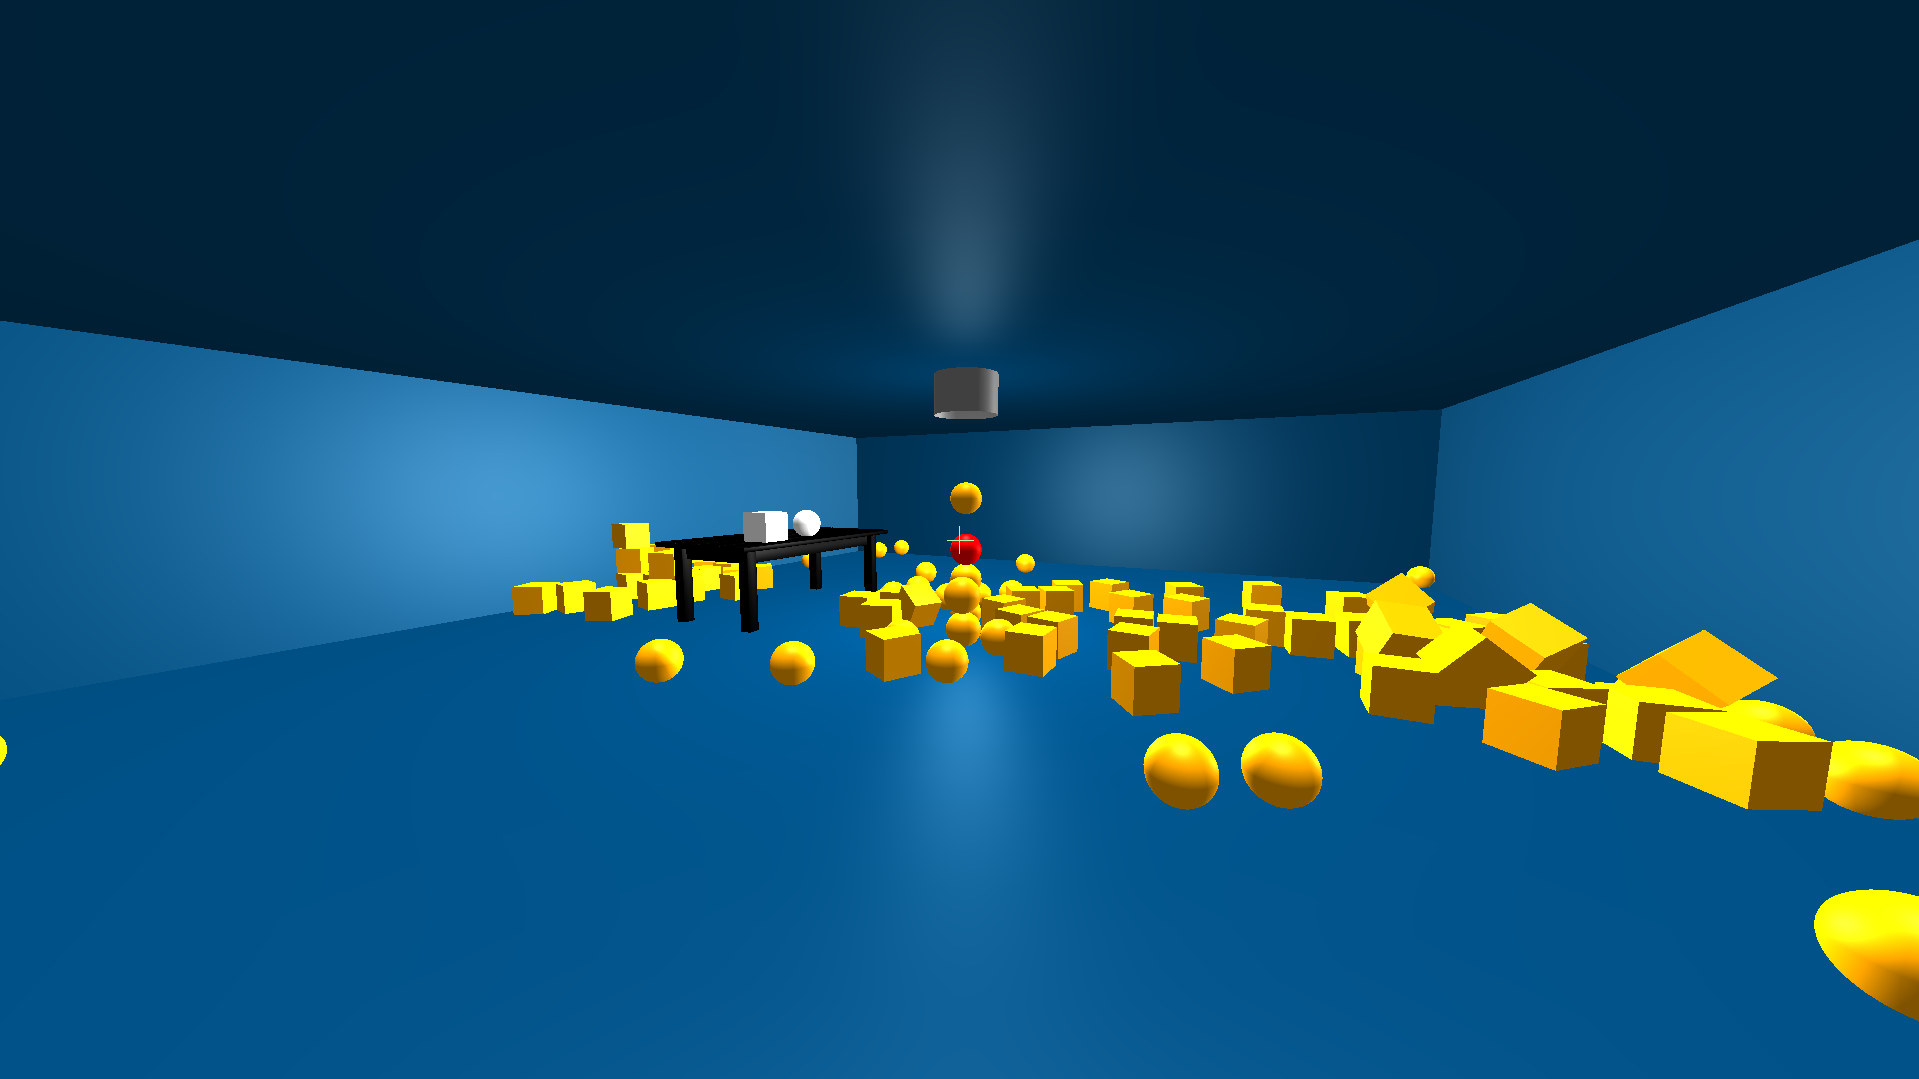
\includegraphics[width=\linewidth]{images/objects.png}

Home room with "doors"

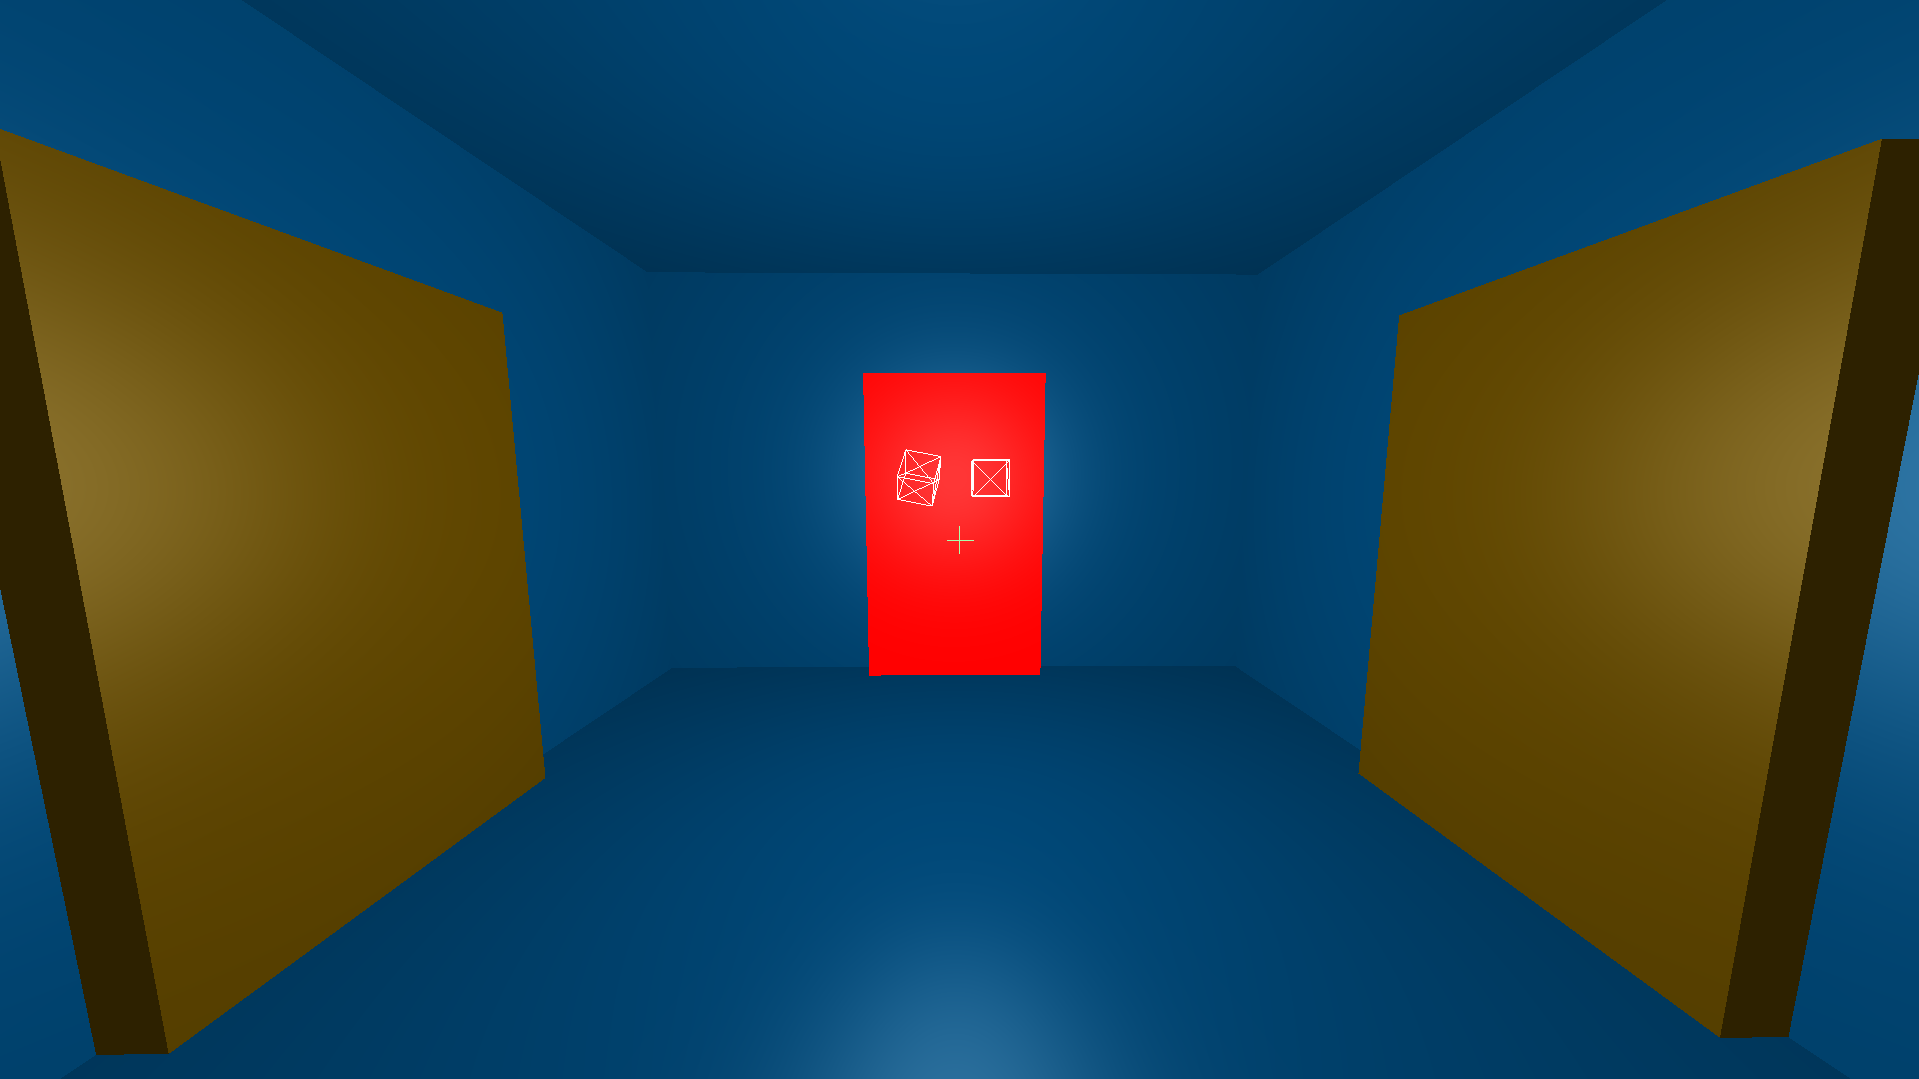
\includegraphics[width=\linewidth]{images/doors.png}

\subsection{Evan}
I've done some 3d modelling for the pendulum experience.  Currently, I have a planet surface, a pendulum, a table, a room with these objects placed and well lit, and a door.  All of these objects have few polygons fulfilling our goals of reaching a broad number of devices.

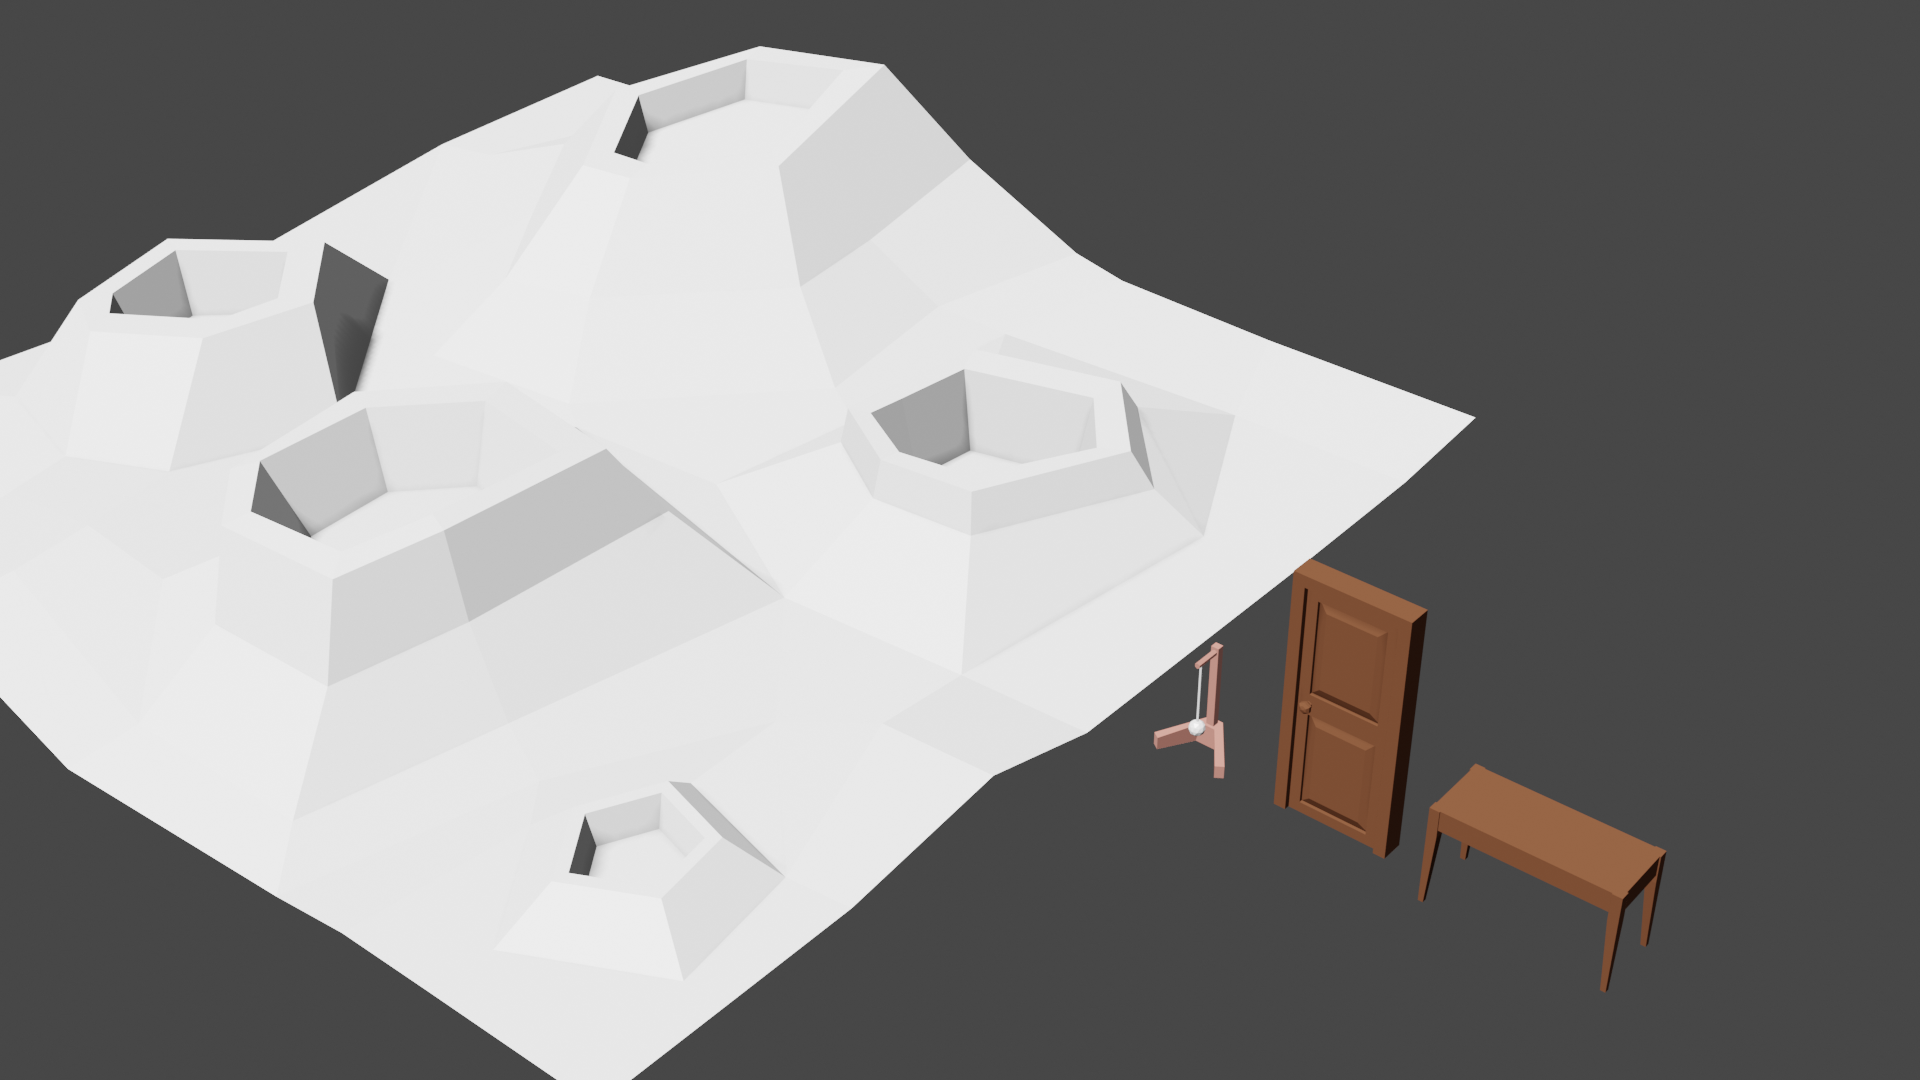
\includegraphics[width=\linewidth]{images/3d_objects.png}

The door will be how users navigate between rooms while in VR.  Currently, users can switch between rooms by exiting the immersive session and using normal links.  The possible navigation endpoints are in our router.js:

\begin{lstlisting}
const Routes = {
  get '/'() {
    return new HomeScene(renderer, camera);
  },
  get '/planets'() {
    return new PlanetsScene(renderer, camera);
  },
  get '/pendulums'() {
    return new PendulumScene(renderer, camera);
  }
};
\end{lstlisting}

The door navigation is functional in the pendulum room.  Selecting it in VR switches to the home scene where more doors are for navigating between the other experiments.

\begin{lstlisting}
// Navigation using links
for (const el of document.links) {
  el.addEventListener('click', (e) => {
    e.preventDefault(); // Stop the browser from navigating to the link's location.
    e.stopPropagation();
    navigate((new URL(el.href)).pathname);
  });
}
// Navigation using doors will look something like:
for (let door of doors) {
    door[Interactions] = {
        select(closeness, {distance, point, face, faceIndex, uv}) {
          navigate('/'); // Navigate to the home room
        }
    };
}
\end{lstlisting}

I also did the initial website styling including the animated arrow, full width and height first page.

My latest work has been building the framework for responding to the 3d equivalents of click and hover events.  Objects can have callbacks for select and hover.  This is an example of how the pendulum swing is setup:

\begin{lstlisting}
// Interactions for the pendulum swing
    const pendulum_swing = importedScene.getObjectByName('Pendulum_Swing');
    pendulum_swing[Interactions] = Object.assign(yellowOnHover(pendulum_swing), {
      drag_start(intersection, pointerMatrix) {
        this.paused = true;
        // this.clearPendulumState();
        const pointerInverse = new Matrix4().getInverse(pointerMatrix, true);
        const target = new Matrix4().copy(intersection.object.matrixWorld);
        const transformMatrix = new Matrix4().multiplyMatrices(pointerInverse, target);
        return {
          object: intersection.object,
          transformMatrix,
          matrixAutoUpdate: intersection.object.matrixAutoUpdate
        };
      },
      drag(matrix) {
        const target = new Vector3().setFromMatrixPosition(matrix);
        const origin = new Vector3().setFromMatrixPosition(pendulum_swing.matrixWorld);
        const transform = new Matrix4().lookAt(origin, target, new Vector3(0, 0, 1));

        const quat = new Quaternion().setFromRotationMatrix(transform);
        quat.z = 0;
        quat.w = 0;
        quat.x *= -1;
        quat.normalize();
        transform.makeRotationFromQuaternion(quat);

        transform.copyPosition(pendulum_swing.matrix);
        pendulum_swing.matrix.copy(transform);
        pendulum_swing.updateMatrixWorld(true);
      },
      drag_end: () => {
        this.calculatePendulumState();
        this.paused = false;
      }
    });
\end{lstlisting}

In addition to the hover and select events, I've been working on drag and drop which allows objects to be moved by the user.  The framework for this also allows for manipulation of that motion.  In the case of the pendulum experiment this means that the pendulum "snaps" to the tables.  In reality, there are five snapping objects in the scene located on each of the tables.  When the user drags the pendulum close to one of these objects it copies the position and rotation onto the pendulum.  When the pendulum is snapped to a table, it updates the equations for swinging the pendulum.  Those equations are also updated when the user moves the pendulum swing.

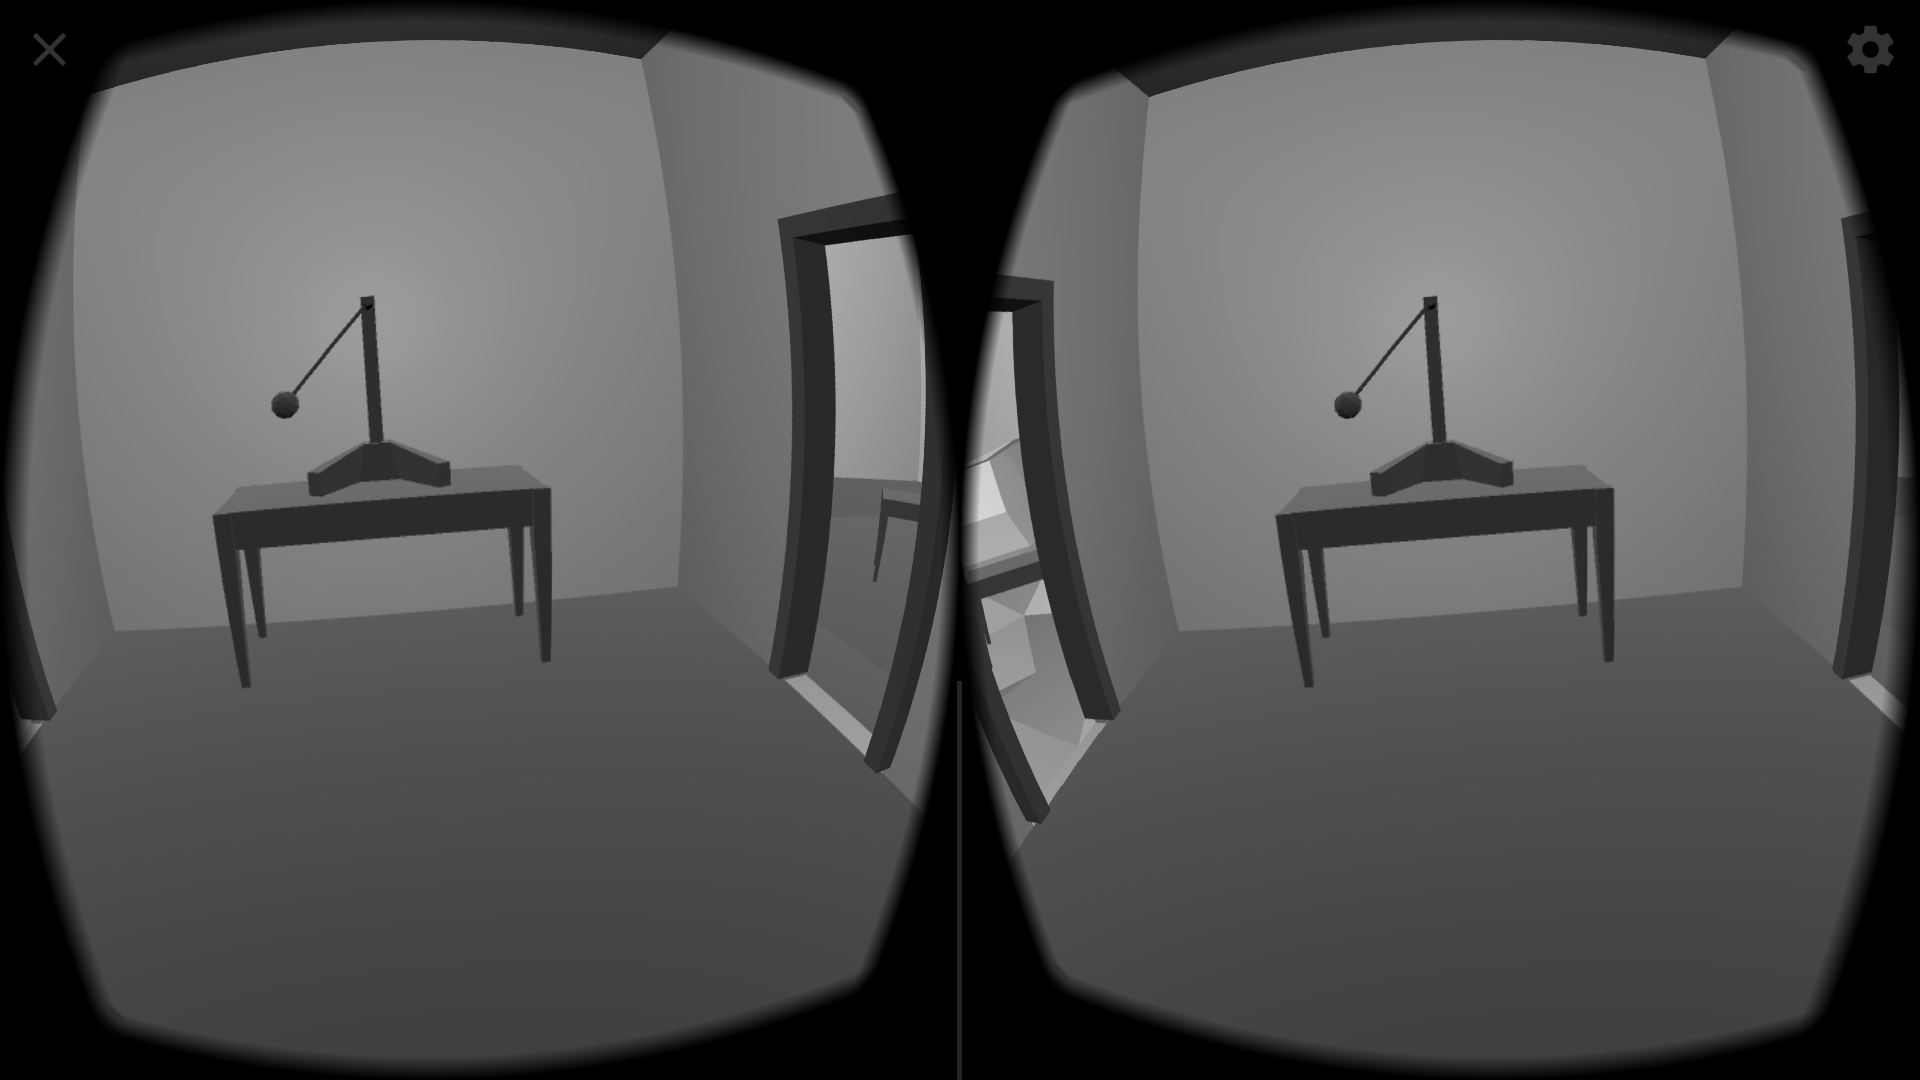
\includegraphics[width=\linewidth]{images/pend-midswing-left.png}

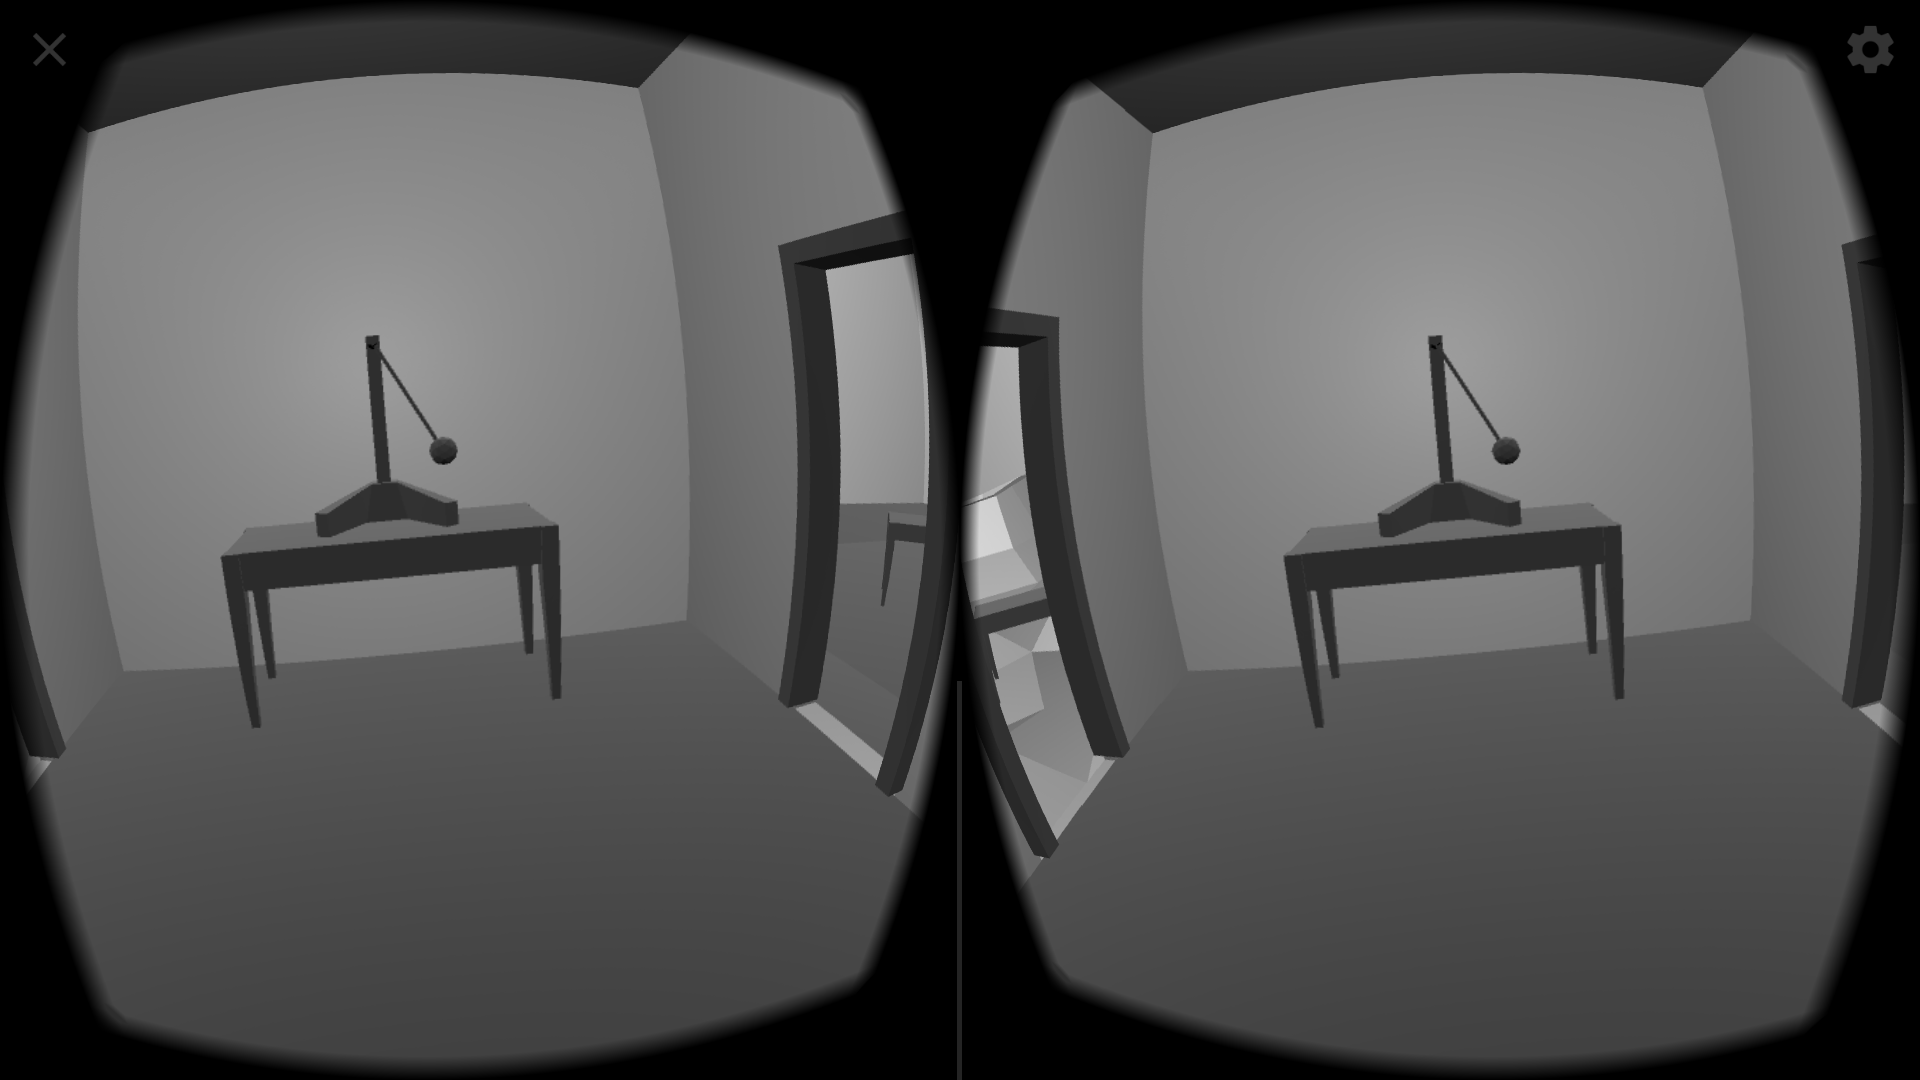
\includegraphics[width=\linewidth]{images/pend-midswing-right.png}

The pendulum swing is joined to the pendulum and moves around with it.  When you try to drag the pendulum swing it stays connected to the pendulum and instead points at the location that you would have placed it at.  This is how the swing's amplitude is set.  When the swing is released it oscillates at the frequency determined by which snapping point and associated gravity it receives.

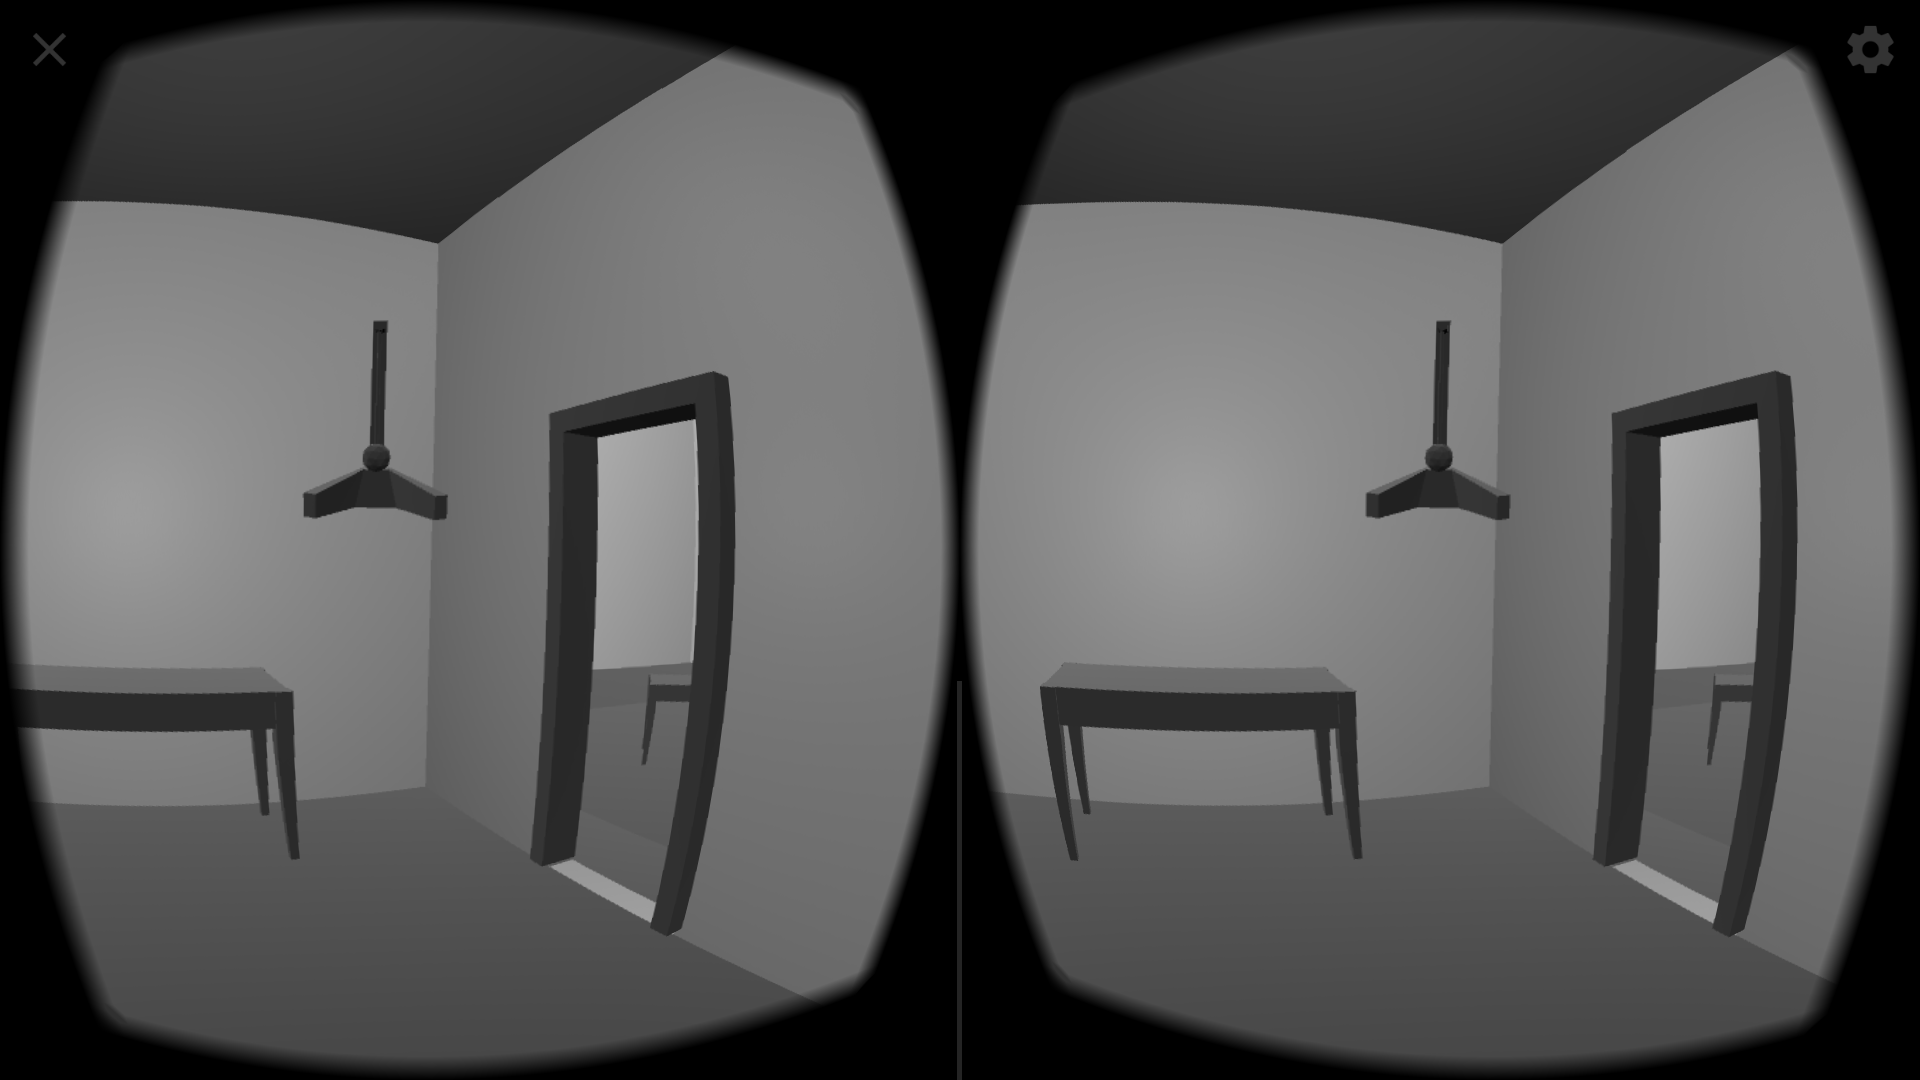
\includegraphics[width=\linewidth]{images/pend-dragged.png}



\subsection{Jonathan}
Over the last few weeks I have been responsible for setting up the Three.js graphical back-end and implementation of the WebXR API in conjunction with the Three.js renderer. My work in Three.js included setting up boilerplate code, a shared parent class among the experiences and a unified animation handler between those rooms. For the WebXR API I was tasked with XR device validation and XR session initialization. This enabled the site to check for XR devices and then set up a magic window or immersive VR rendering session. I also set up event listeners for a VR button that allowed the user to activate/create an immersive VR session on click. Near the end of the term I completed the implementation of the WebXR API by setting up XR input controller/ray rendering and XR/Standard input event handling.

    \subsubsection{Progress}
    
    For the first couple of weeks, I spent my time tinkering with the Three.js code looking for a way to make sure that all the experience rooms would cooperate with each other in runtime. Along with Brooks, we decided on a structure in which all experience rooms are derived from one parent class that shares a renderer and animation handler. This allows us to easily switch between different rooms by constructing them from the parent class on each room switch event. The shared renderer also provides a seamless transition between experience rooms and the unified animation handler ensures that each new room can easily begin rendering frames on creation. 
    
    While setting up the unified animator, we ran into an issue where the animation loops of previous rooms continued executing even after the room had changed. This was solved by setting an isActive value for each room instance. Later on, I added a restart animation function that would stop execution of the current animation loop then start it up again. This was implemented in response to an issue where XR sessions would automatically end the current animation loop. For some XR sessions, it's required that the animation loop is manually started up again on its creation. There were some other cases though where the XR session would start a second animation loop. The cancel animation frame code was added to handle events in which a frame had already been in the render loop.
    \begin{lstlisting}
  /**
   * Override this to handle animating objects in your scene.
   * @param {number} delta time since last scene update
   */
  animate(delta) {
    return delta;
  }

  /**
   * Call this to begin animating your frame.
   */
  startAnimation() {
    this._animationCallback();
  }

  _restartAnimation = () => {
    if (this.frame) window.cancelAnimationFrame(this.frame);
    this._animationCallback();
  };

  _animationCallback = (timestamp, xrFrame) => {
    if (this.isActive) {
      // Update the objects in the scene that we will be rendering
      const delta = this.clock.getDelta();
      this.animate(delta);
    \end{lstlisting}
    
    The majority of my time over the last few weeks was spent implementing the WebXR API. There were many challenges to overcome. First of all was the instability of the API and its unreliable polyfill. Under the direction of the client, I started this process using the WebXR polyfill. This was a mistake. The polyfill is not nearly as reliable as the most current version of WebXR. Though it is a polyfill, oftentimes the functions I needed to call were unsupported and out of date. After some discussion with the client, I stopped using the polyfill.
    
    The up-to-date API was not without its issues. As it is brand new and unstable, we are required to use the most up-to-date version of Chrome Dev/Canary for testing/deployment and often, many of the code snippets we write are unreliable and may be unusable at any time. For this reason, we are constantly having to keep an eye on the WebXR API and Chrome updates.
    
    The WebXR session validation is a multi-step process that begins with checking if the current device is capable of non-immersive sessions. A non-immersive session is one in which XR properties of the device are read, but are only used in a single rendering context. This is also called magic window rendering, a session primarily used on mobile devices. Most modern mobile devices can support these types of sessions and will pass the checks that I have written.
    
    Before a magic window session is created, a new xrpresent rendering context needs to be created. Normally, a WebGL rendering context is used and this is what our main rendering canvas uses. Unfortunately, once a rendering context has been attached to a canvas, it can no longer be changed. Instead, a new canvas is created with the correct rendering context and added to the DOM. Once that canvas has been created, the WebXR API navigator makes a request for a non-immersive session using the rendering context we've just created. 
    \begin{lstlisting}
/**
 * Checks for magic window compatibility
 */
async function xrValidateMagicWindow() {
  // Ensure that there isn't already a magic window
  if (!XR.magicWindowCanvas) {
    XR.magicWindowCanvas = document.createElement('canvas');
    XR.magicWindowCanvas.setAttribute('id', 'vr-port');
    XR.magicWindowCanvas.setAttribute('name', 'magic-window');
    canvas.parentNode.insertBefore(XR.magicWindowCanvas, canvas);
  }
  XR.magicWindowCanvas.width = window.innerWidth;
  XR.magicWindowCanvas.height = window.innerHeight;

  // Set canvas rendering context to xrpresent
  const xrMagicWindowContext = XR.magicWindowCanvas.getContext('xrpresent');

  try {
    XR.session = await navigator.xr.requestSession({ outputContext: xrMagicWindowContext });
    canvas.style.display = 'none';
    xrOnSessionStarted();
  } catch (reason) {
    XR.magicWindowCanvas.style.display = 'none';
    console.log(`Device unable to support magic window session : ${reason}`);
  }
}
    \end{lstlisting}
    
    When requesting an immersive session, the process is similar to magic window validation.
    \begin{lstlisting}
/**
 * Gets an immersive two eye view xr session when the 'ENTER XR' button has been pressed
 */
async function xrOnRequestSession() {
  // Create a mirror canvas for rendering the second eye
  const xrMirrorCanvas = document.createElement('canvas');
  const xrMirrorContext = xrMirrorCanvas.getContext('xrpresent');
  xrMirrorCanvas.setAttribute('id', 'mirror-canvas');

  // Add the mirror canvas to our XR object and the document.
  XR.mirrorCanvas = xrMirrorCanvas;
  document.body.appendChild(xrMirrorCanvas);

  // Attempt to create an XR session using the mirror canvas and the connected device
  try {
    XR.session = await navigator.xr.requestSession({ mode: 'immersive-vr', outputContext: xrMirrorContext });
    xrOnSessionStarted();
  } catch (err) {
    console.error(`Error initializing XR session : ${err}`);
  }
}
    \end{lstlisting}
    
    Once the XR session has been created, I export an XR object that contains all the necessary information to render a single frame. The session object, the frame of reference from which XR input is written and the two rendering canvases.
    \begin{lstlisting}
export const XR = {
  session,
  immersiveRefSpace,
  nonImmersiveRefSpace,
  magicWindowCanvas,
  mirrorCanvas
};
    \end{lstlisting}
    
    In the unified animator, I query the reference space for its pose. The pose holds all the XR views, these views hold their rendering viewports and the transformation matrices for each XR object in the scene. I used this information to manually update the three.js camera and scene matrices to reflect the positioning of the XR device.
    \begin{lstlisting}
for (let i = 0; i < pose.views.length; i++) {
  const view = pose.views[i];
  const viewport = XR.session.renderState.baseLayer.getViewport(view);
  const viewMatrix = new Matrix4().fromArray(view.viewMatrix);

  this.renderer.context.viewport(
    viewport.x,
    viewport.y,
    viewport.width,
    viewport.height
  );

  // Update user position if touch controls are in use with magic window.
  if (XR.magicWindowCanvas && XR.magicWindowCanvas.hidden === false) {
    updateTouchPosition(viewMatrix);
    this._translateViewMatrix(viewMatrix, userPosition);
    } else {
      this._translateViewMatrix(viewMatrix, new Vector3(0, 0, 0));
    }

    this.camera.matrixWorldInverse.copy(viewMatrix);
    this.camera.projectionMatrix.fromArray(view.projectionMatrix);
    this.scene.matrix.copy(viewMatrix);

    this.scene.updateMatrixWorld(true);
    this.renderer.render(this.scene, this.camera);
    this.renderer.clearDepth();
}
    \end{lstlisting}
    
    Once the XR view rendering was complete, users could experience our site in standard, magic-window and immersive view sessions. The next logical step was to begin implementing the WebXR input interface. Just like the view devices, the WebXR API gets a 'pose' for each connected input device. This includes touch in magic-window and gaze/controller rays in immersive sessions. For sessions without a controller, WebXR gets the pose of a target ray. This is a virtual ray that is projected into the scene from touch events, gaze and XR controllers. Sessions that have an XR controller device connected will also provide a grip pose which describes the transformations of the connected input device.
    
    Using the grip pose data, I was able to render a controller into the scene that emulated the position and rotation of the XR input controller in real life. An issue that I ran into immediately was keeping track of the connected input devices and updating their mesh positions in the scene. In an XR session there can be 0 to 2+ input devices connected at any one time. I needed a way to keep track of each controller and its associated mesh in the scene. To solve this issue I created a controller class which held information about the controller mesh, its associated laser and the functions necessary for updating those meshes every frame. Then for every frame, I checked the number of controllers I was keeping track of versus the number of input sources that the WebXR API was tracking and then added/removed controllers appropriately by adding them to an array in our xrScene class.
    \begin{lstlisting}
if (isTrackedPointer && inputSource.gripSpace) {
  // Get grip space pose for controller
  const gripPose = xrFrame.getPose(inputSource.gripSpace, xrRefSpace);

  // Is the number of controllers we know of less than the number of input sources?
  if (this.controllers.length > inputSources.length) {
    // Remove controller from array if number of controllers
    // is less than number of input sources
    this._removeController(i);
  } else {
    if (this.controllers.length < inputSources.length) {
      // Create a new controller and add to the scene
      const controller = new Controller(this.controllerMesh.clone());
      this.controllers.push(controller);
      this.scene.add(controller.mesh);
    }

    // Get the grip transform matrix
    const gripMatrix = new Matrix4().fromArray(gripPose.transform.matrix);

    // Make sure to translate the controller matrix to the user position
    this._translateObjectMatrix(gripMatrix, userPosition);

    // Apply grip transform matrix to the current controller mesh
    const matrixPosition = new Vector3();
    gripMatrix.decompose(matrixPosition, new Quaternion(), new Vector3());
    this.controllers[i].updateControllerPosition(gripMatrix);
  }
}
    \end{lstlisting}
    
    Once the controller was rendered into the scene correctly, I began creating a framework for object interactions. Since there would be multiple types of sessions that the user could experience, we either needed a raycaster for every session or one single raycaster to handle it all. Of course, I wanted to create a raycaster that we could all use across every session for every situation. I began by creating a file to hold a global raycaster and wrote some functions that could be used to update its ray, and return its current intersections in the scene.
    
    There are examples all over the place of how to implement a raycaster using mouse/keyboard in Three.js on the web but there are little to no examples for how to raycast using Three.js in a WebXR session. Let alone any examples using some unified raycaster. Figuring out how to structure every frame to handle the raycaster updating from non-XR and XR sessions in addition to firing events for every type of user gesture was hard to say the least.
    
    The first big hurdle that I had to overcome was updating the raycaster's ray from the XR input source. Not did I have to take into account the XR input device, but I also had to handle changes in the world matrix from the viewing device rotations. The solution for this was to implement code that shared many similarities with the view updating code. One issue though was that at this point in the program, I had lost my reference to the new view matrix. This was easily solved by using the scene object's matrixWorld that held the most up to date changes to the rendered scene. Once I got that sorted out, I was able to place the ray's origin correctly but the ray's direction was still skewed. The solution to this was to create a default directional vector that pointed in the negative Z direction (Where we are always looking by default) and then transform it by the direction of the transformed target ray matrix direction.
    \begin{lstlisting}
/**
* Calculates raycast intersections on a frame by frame basis
* from the XR target rays. Triggers the respective events for
* each intersection based on the current state of the input ray
* and trigger object.
* @param {Matrix4} targetRayMatrix Transformation matrix from the
* XR input pose
* @returns {Intersection} Intersection info, this can be null
*/
_raycastIntersection(targetRayMatrix) {
const trMatrix = new Matrix4().fromArray(targetRayMatrix);
this._translateObjectMatrix(trMatrix, userPosition);

// Transformed ray matrix from the current scene matrix world
const rMatrix = new Matrix4().multiplyMatrices(this.scene.matrixWorld, trMatrix);
// Ray origin vector derived from the ray matrix
const rOrigin = new Vector3().setFromMatrixPosition(rMatrix);

// Orientation for ray on -Z Axis transformed and normalized by the ray matrix
const rDest = new Vector3(0, 0, -1).transformDirection(rMatrix)
  .normalize();

// Update raycaster object orientation
updateRay(rOrigin, rDest);

// Handle intersection events
return this._intersectionHandler();
}
    \end{lstlisting}
    
    Now that the raycaster was projecting rays correctly in the scene, I need to find some way to handle user gestures and interactions. I needed some sort of logic structure that would be able to interpret exactly what the user was trying to do for every frame. This boiled down to about four things. Hovering, selecting (holding), releasing and exiting (leaving the hover). I also needed to make sure that only certain objects were available for interaction and that each object would be capable of reacting to an event in different ways.
    
    To allow objects to react differently from one another to interaction events, I created a new Three.js Mesh class called TriggerMesh. A TriggerMesh inherits from a Mesh but has four functions inside of it that can be called on each type of interaction event. Those functions do some default behavior and then call a special functions that can be defined differently for each object (see Tim's example).
    \begin{lstlisting}
/**
 * Called when raycaster is currently intersecting
 * Called every frame onHover
 * @param {Intersection} intersection
 */
onTriggerHover(intersection) {
  if (this.debug) console.log('TRIGGER: HOVER');
  this.isIntersected = true;
  if (this.hover) this.hover(intersection);
}

/**
 * Called when raycaster no longer intersects
 * this object.
 * Called once on exit.
 * @param {Intersection} intersection
 */
onTriggerExit(intersection) {
  if (this.debug) console.log('TRIGGER: EXIT');
  this.isIntersected = false;
  if (this.exit) this.exit(intersection);
}

/**
 * Called when raycaster intersects and
 * the input device clicks and holds.
 * Called every frame on selection.
 * @param {Intersection} intersection
 */
onTriggerSelect(intersection) {
  if (this.debug) console.log('TRIGGER: SELECT');
  this.isSelected = true;
  if (this.select) this.select(intersection);
}

/**
 * Called when raycaster input device
 * releases a click when intersecting.
 * Called once on release.
 * @param {Intersection} intersection
 */
onTriggerRelease(intersection) {
  if (this.debug) console.log('TRIGGER: RELEASE');
  this.isSelected = false;
  if (this.release) this.release(intersection);
}
    \end{lstlisting}
    
    With the TriggerMesh, I was ready to start handling intersections. I created the logic structure and placed it somewhere where it could be called every frame. The result was a perfectly executed user interaction session in all forms of experiences in our site.
    \begin{lstlisting}
/**
* Gets an intersection from the raycaster and fires
* the appropriate events in response to certain
* user gestures and ray orientation
*/
_intersectionHandler() {
// Get nearest trigger object intersection from raycaster
const intersection = getIntersection(this.triggers);

if (intersection) {
  // Ensure that keyboard/mouse is not enabled before applying inverse world matrix to point
  if (!(controls && controls.enabled)) {
    // Fix the intersection point as it is in world coordinates
    // rather than scene local coordinates
    intersection.point.applyMatrix4(new Matrix4().getInverse(this.scene.matrixWorld));
  }

  intersection.object.onTriggerHover(intersection);
  if (!intersection.object.isSelected) {
    if (this.buttonPressed) {
      // Previous frame was not selected but user is pressing button
      intersection.object.onTriggerSelect(intersection);
      // Keep track of selected object reference
      this.selected = intersection.object;
    }
  } else if (!this.buttonPressed) {
    // Trigger object WAS selected but button is now longer pressed
    intersection.object.onTriggerRelease(intersection);
    // Drop selected object reference on release of selection
    this.selected = null;
  }
}
return intersection;
}
    \end{lstlisting}
    
    \subsubsection{Visuals}
    Magic Window
    
    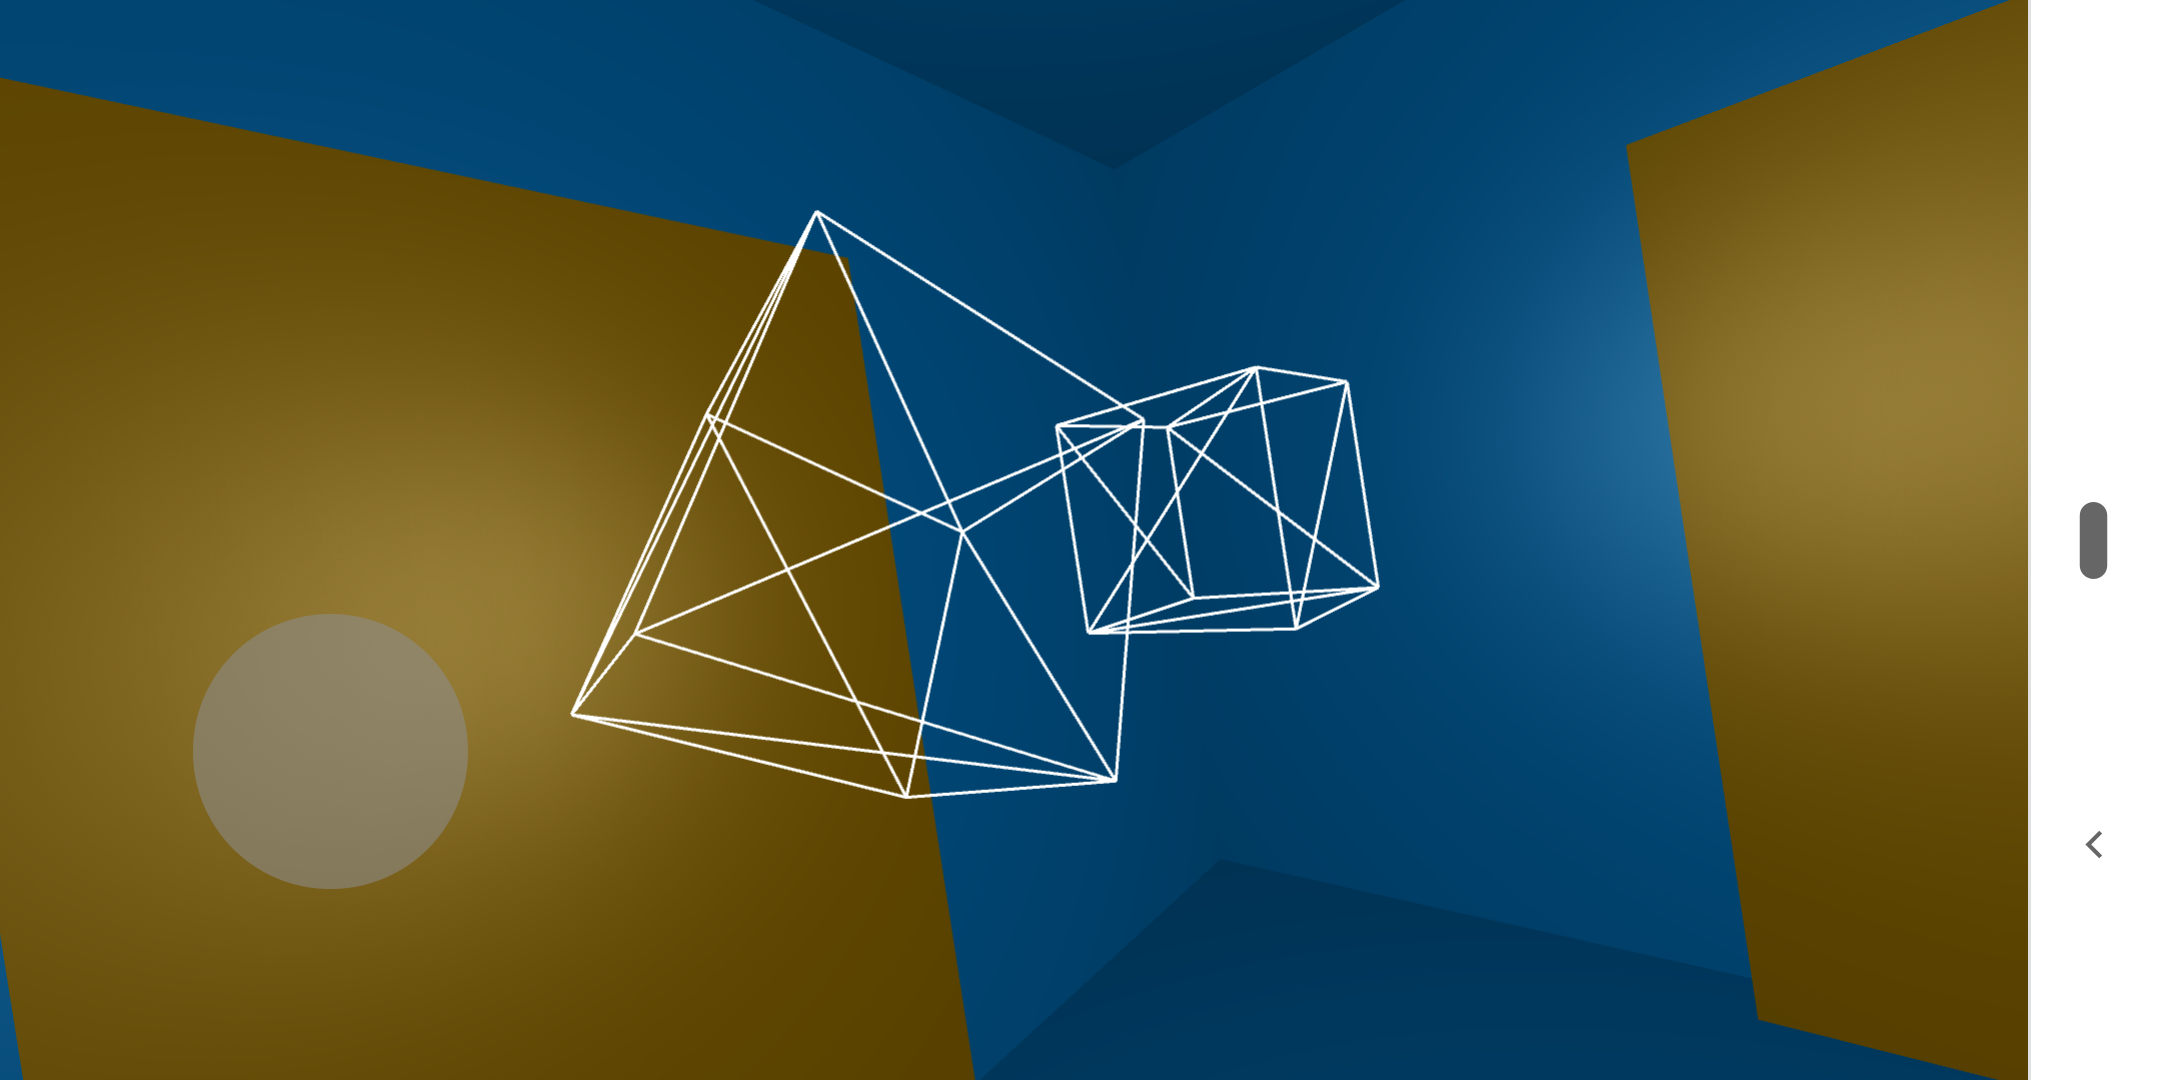
\includegraphics[width=\linewidth]{images/MagicWindow.png}
    
    Immersive View
    
    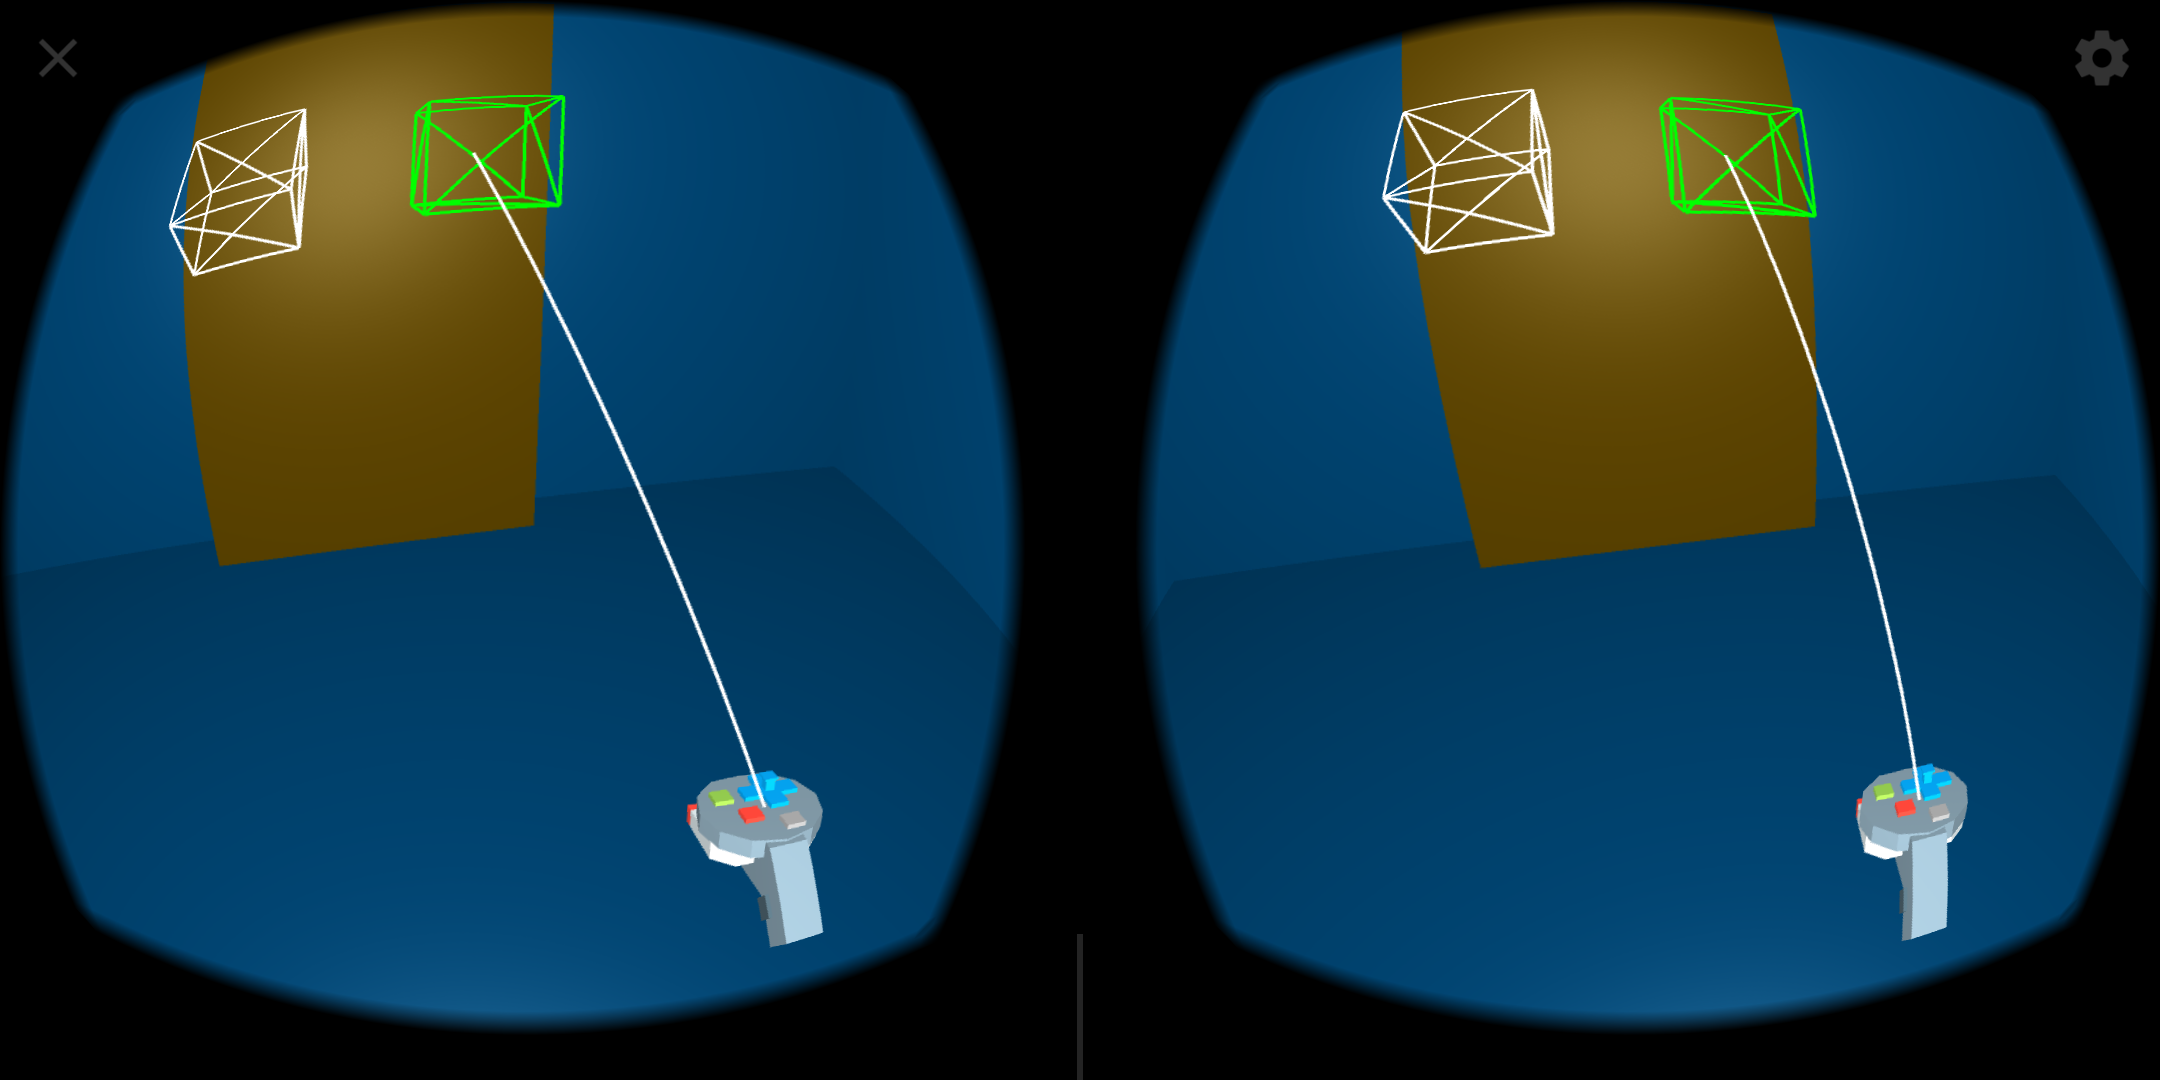
\includegraphics[width=\linewidth]{images/ImmersiveView.png}
    
\subsection{Brandon}
   For the couple of weeks I have been tasked for setting up Cannon.js. My work started with setting up a basic room using Three.js that could later used when setting up a Lightweight 3D physics for the web. I began with the creation of a cannon world object.
   
   \subsubsection{Progress}
   First, I begin creating a cannon world that is the physics hub that manage objects and simulation. Then I set the gravity to be in the negative y direction and I added a broadphase algorithm to the world so it can easily find colliding bodies. This will set up the physics world and the next part is adding objects to it. The bodies are built once you define a shape, a rigid body using the shape and other physical properties needed, and then add the body to the world. I created a spherical shape with a radius of 1 so it can be put into a rigidbody before it can move and collide. Next I create a rigidbody and set the body mass to 1 so it makes the sphere dynamic. If the mass is set to zero it becomes static amd static don't collie with other static bodies. While dynamic ones collie with all other bodies. Lastly, I add the body to the world so it will move according to the forces it is subject to, and collide with other objects:
   
   \begin{lstlisting}
    const world = new CANNON.World();
    world.gravity.set(0,-15,0);
    world.broadphase = new CANNON.NaiveBroadphase();
    const radius = 1
    const sphereBody = new CANNON.Body(
      {
        mass: 1,
        position: new CANNON.Vec3(1, 0, 0),
        shape: new CANNON.Sphere(radius)
      }
    );
    sphereBody.position.set(0, 5, -5);
    this.world.add(sphereBody);
   \end{lstlisting}
   
   This will create the plane shape, and then the body. I give the body zero mass, this will make sure the ground body to become static. The orientation of the plane I set in a 90 degree angle: 
   
   \begin{lstlisting}
    const groundShape = new CANNON.Plane();
    const groundBody = new CANNON.Body({ mass: 0 });
    groundBody.addShape(groundShape);
    groundBody.quaternion.setFromAxisAngle(new CANNON.Vec3(1, 0, 0), -Math.PI / 2);
    groundBody.position.set(0, -8, 0);
    this.world.addBody(groundBody);
    this.world.add(sphereBody);
    const body = sphereBody;
    return body;
   \end{lstlisting}
    
    After we have initialized the static ground plane and a dynamic sphere. I then set a time step for Cannon.js. Cannon.js uses a computation algorithm to called integrators to simulate the physics equations at a discrete points of time. This step at least 60hz or 1/60 seconds to begin the simulation loop:
   \begin{lstlisting}
   animate() {
   this.updatePhysics();
   this.ball.position.copy(this.body.position);
   this.ball.quaternion.copy(this.body.quaternion);
   }
   \end{lstlisting} 
   
     Next, I started working on a flexible graphical user interface for changing variables by setting up dat.GUIVR to create a 3D interface that you can use within Three.js. I began taking Tim Kinematic motion experience that creates spawn-able objects and implement it with a GUI that is an Object3D. It can be easily position, rotate, or be scaled. The code below creates a menu GUI in the scene. I also enable mouse input for non-VR and a gaze input so testing without a VR device would be easier. 
     
    \begin{lstlisting}
    export default function createGUI(scene, camera, object, world) {
    // Allow mouse input for non-VR app and testing without a VR device.
    dat.GUIVR.enableMouse(camera);

    // Gaze Input is use for on VR devices without controllers.
    const gazeInput = dat.GUIVR.addInputObject(camera);
    scene.add(gazeInput.cursor);

    // Bind mouse or touch on the GUI to a press.
    ['mousedown', 'touchstart', 'keydown']
      .forEach((e) => {
        window.addEventListener(e, () => {
          gazeInput.pressed(true);
        }, false);
      });

    ['mouseup', 'touchend', 'keyup']
      .forEach((e) => {
        window.addEventListener(e, () => {
          gazeInput.pressed(false);
        }, false);
      });

    // Create name test to show at the top of the gui tab.
    const gui = dat.GUIVR.create('Settings');
    gui.position.set(3, 0.5, -13);

    // Set the size of the gui.
    gui.scale.set(2, 2, 2);

    // Gravity Slider.
    gui.add(world.gravity, 'y', -9.8, 9.8).step(0.2)
      .name('Gravity')
      .listen();

    // Track object position.
    gui.add(object.position, 'x').min(-1)
      .max(1)
      .step(0.25)
      .name('Position X')
      .listen();

    gui.add(object.position, 'y').min(-1)
      .max(1)
      .step(0.25)
      .name('Position Y')
      .listen();

    gui.add(object.position, 'z').min(-1)
      .max(1)
      .step(0.25)
      .name('Position Z')
      .listen();

    // Toggle for specific object material as wireframe.
    gui.add(object.material, 'wireframe')
      .name('Wireframe')
      .listen();

    scene.add(gui);
   }
   \end{lstlisting} 
    

    \newpage
    The gravity part is an constraining input can specify limits on numbers. It is a slider that can have a min and max value. An example code below is a gravity slider that has a min value of -9.8 and max 9.8 for gravity. This will allow users to change gravity to the scene.
    
   \begin{lstlisting}
    // Gravity Slider.
    gui.add(world.gravity, 'y', -9.8, 9.8).step(0.2)
      .name('Gravity')
      .listen();
   \end{lstlisting}
 
   \subsubsection{Visuals}
   Sphere position set.
   
   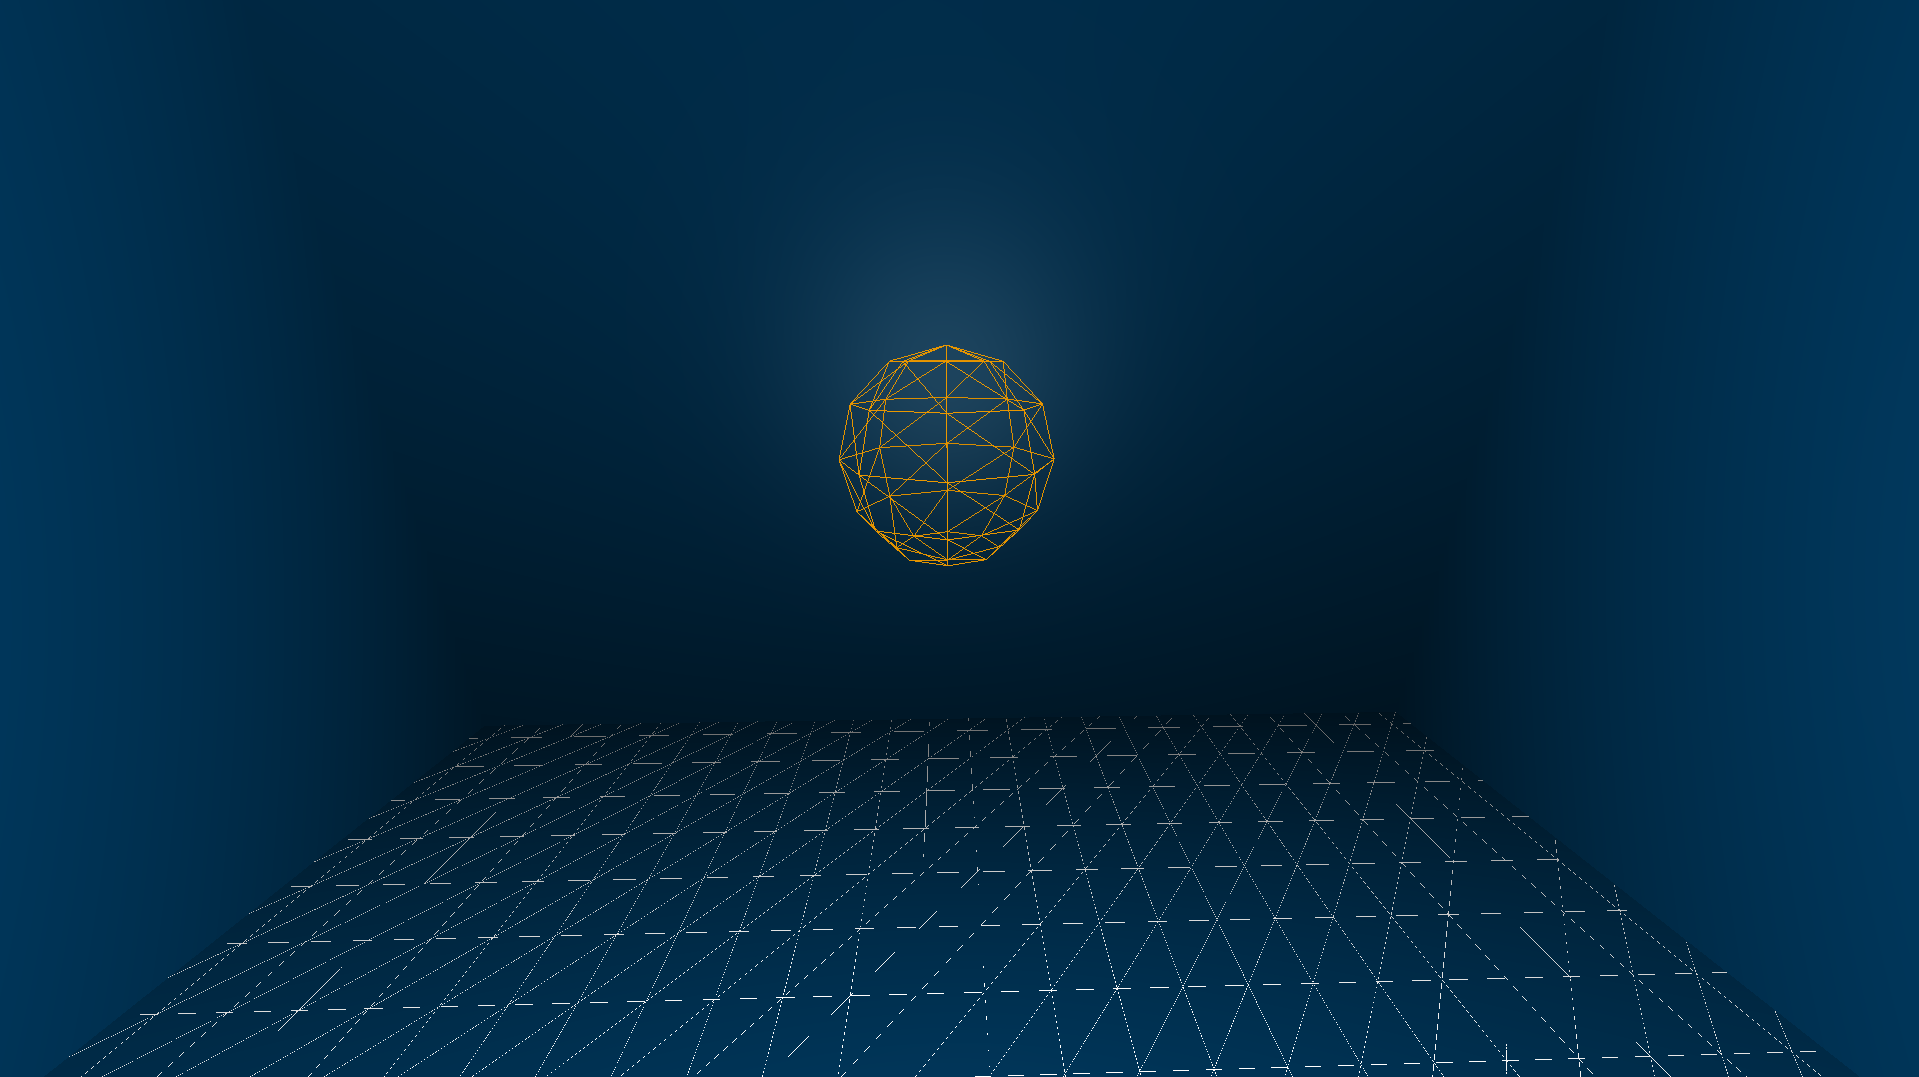
\includegraphics[width=\linewidth]{images/Cannonjs.png}
   
   \newpage
   
   Sphere simulate drop.
   
   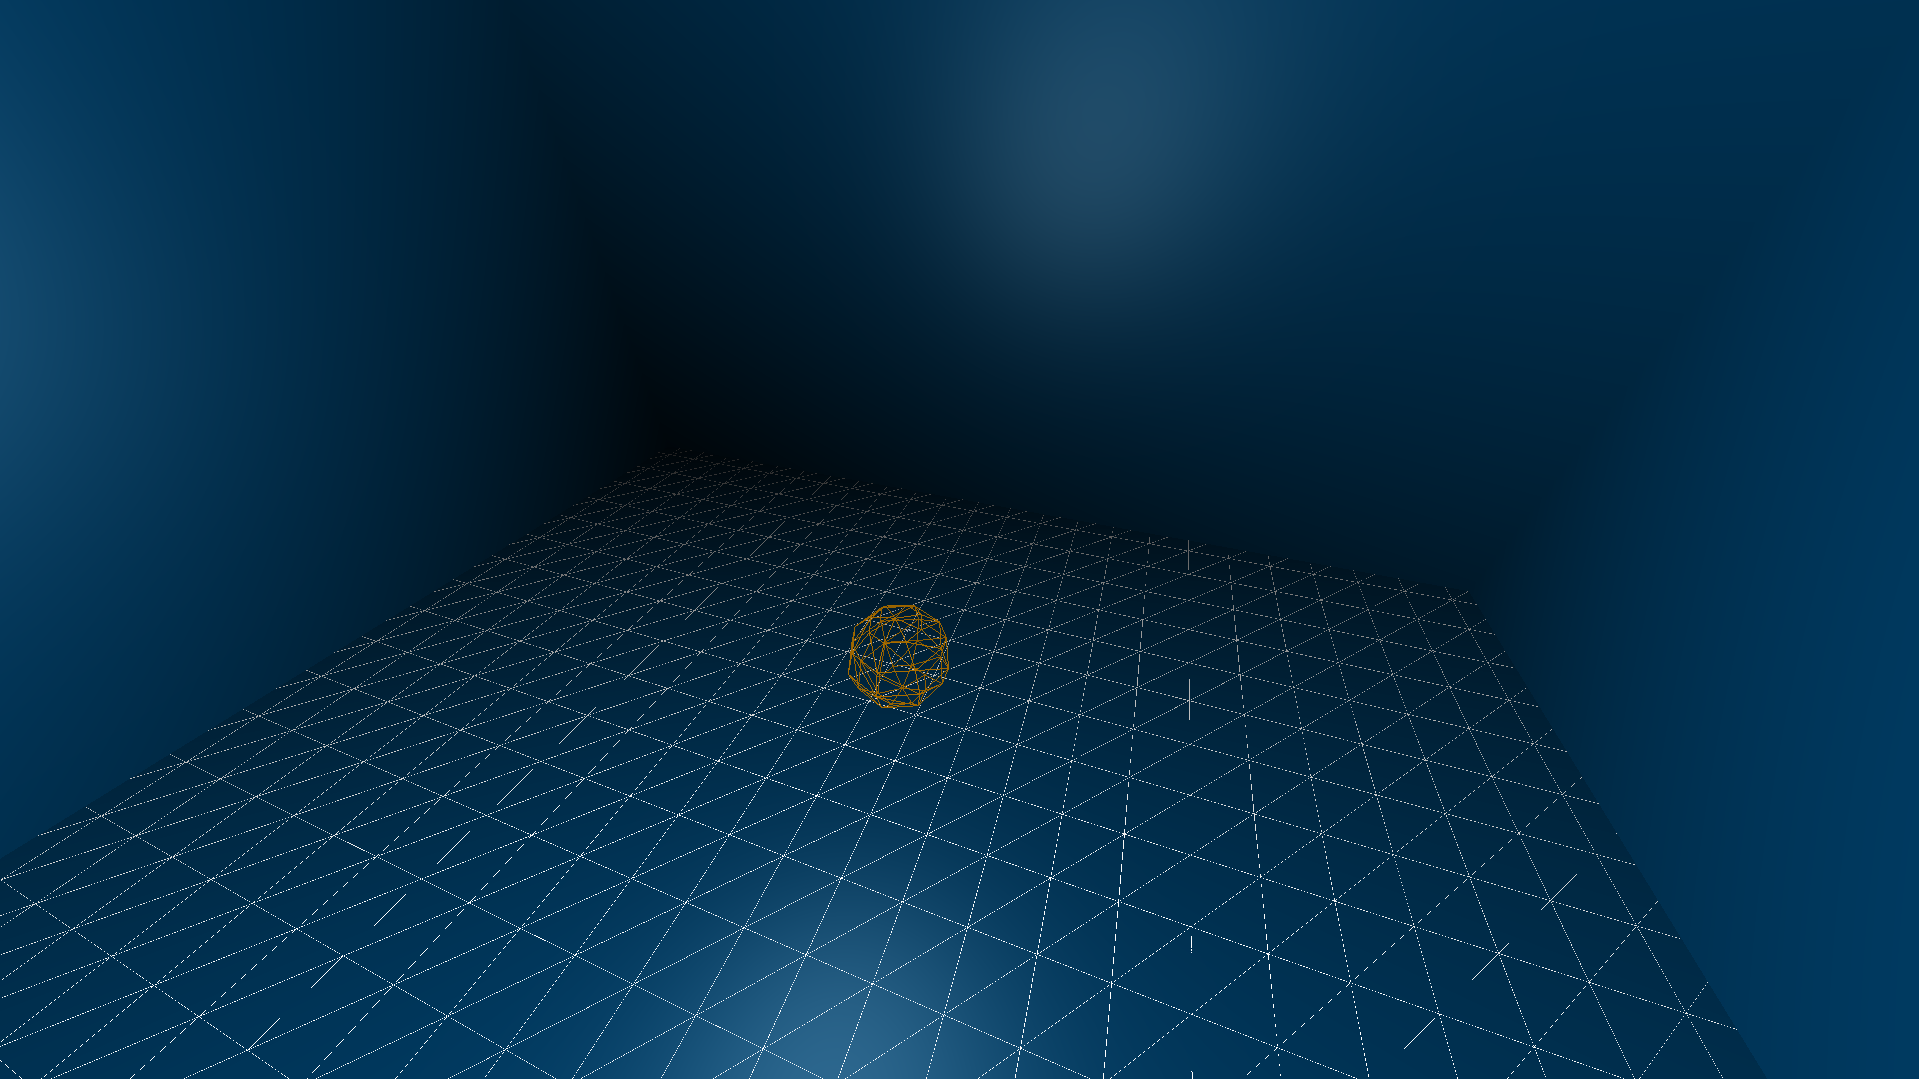
\includegraphics[width=\linewidth]{images/CannonjsDrop.png}
   
   Default position of the 3D object menu interface.
   
   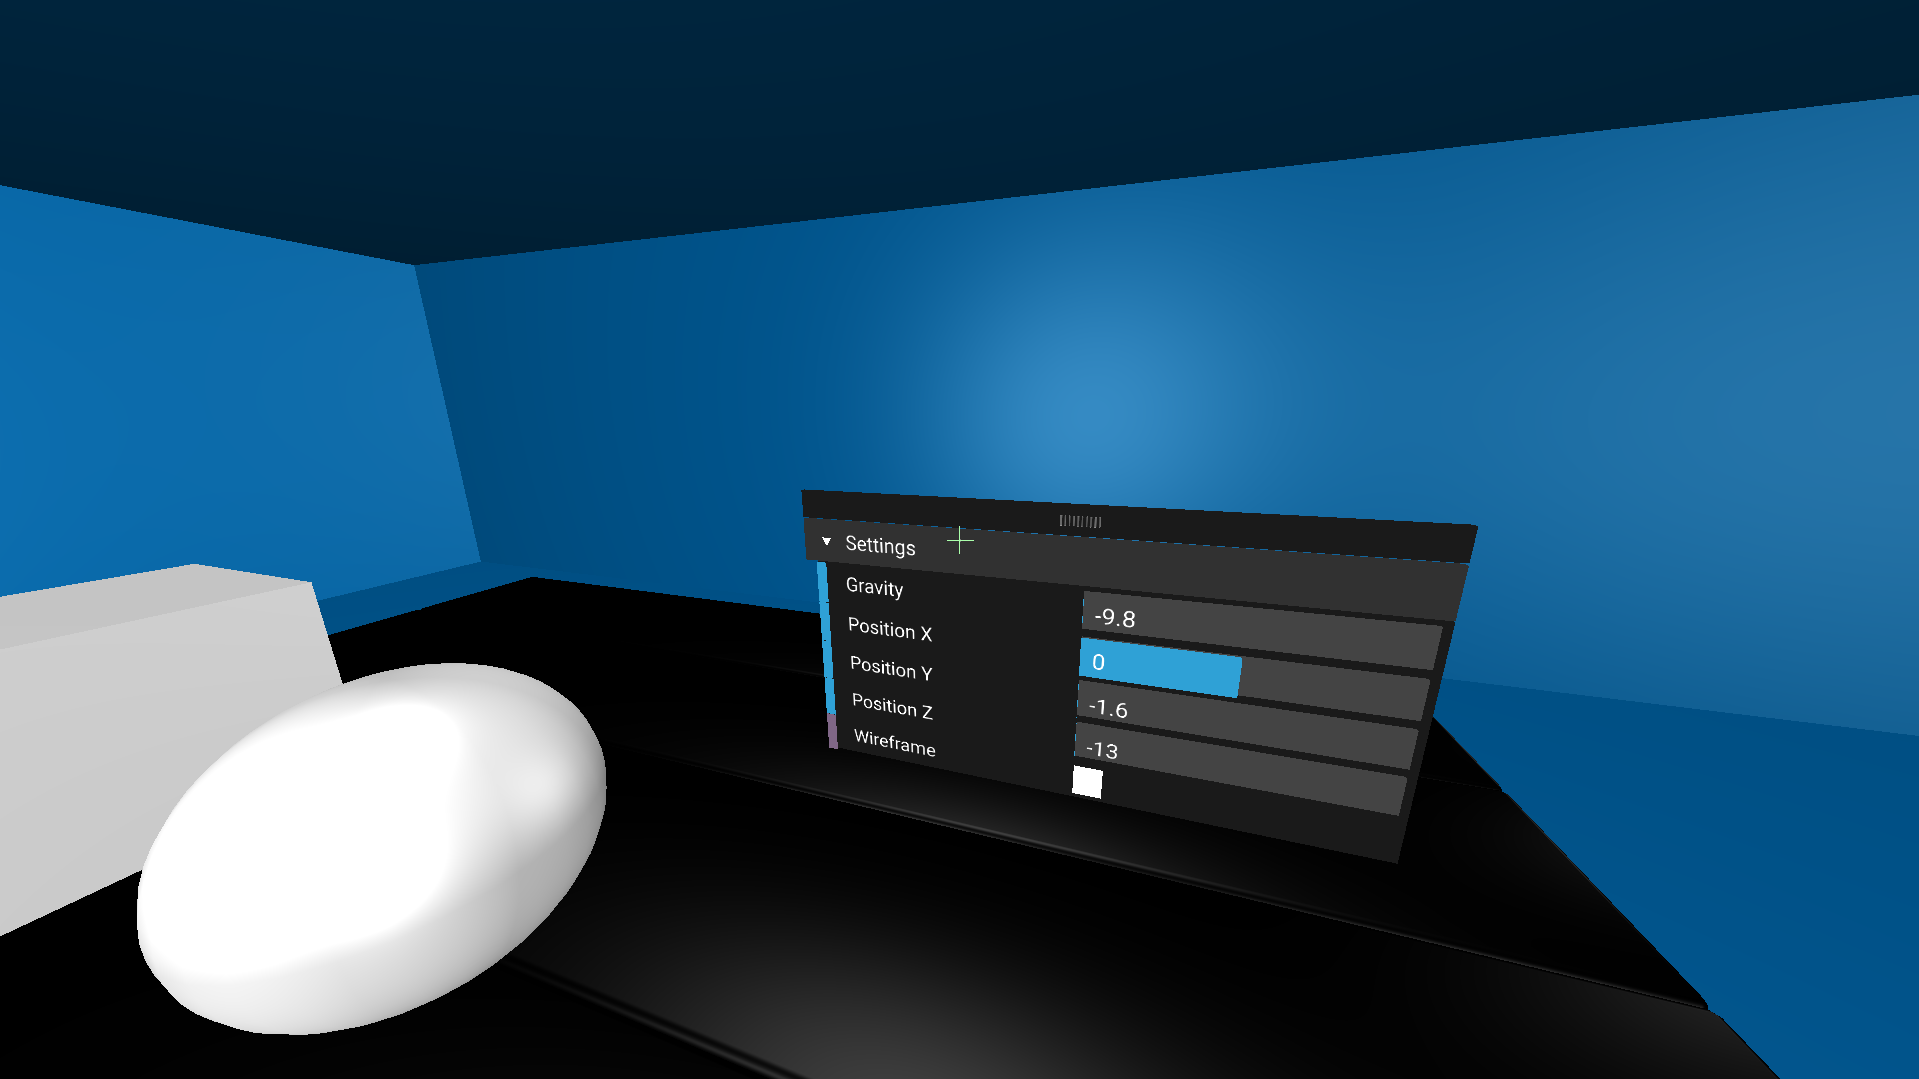
\includegraphics[width=\linewidth]{images/menu-gui.png}
   
   Spawn bunch of objects and set gravity to 0.
   
   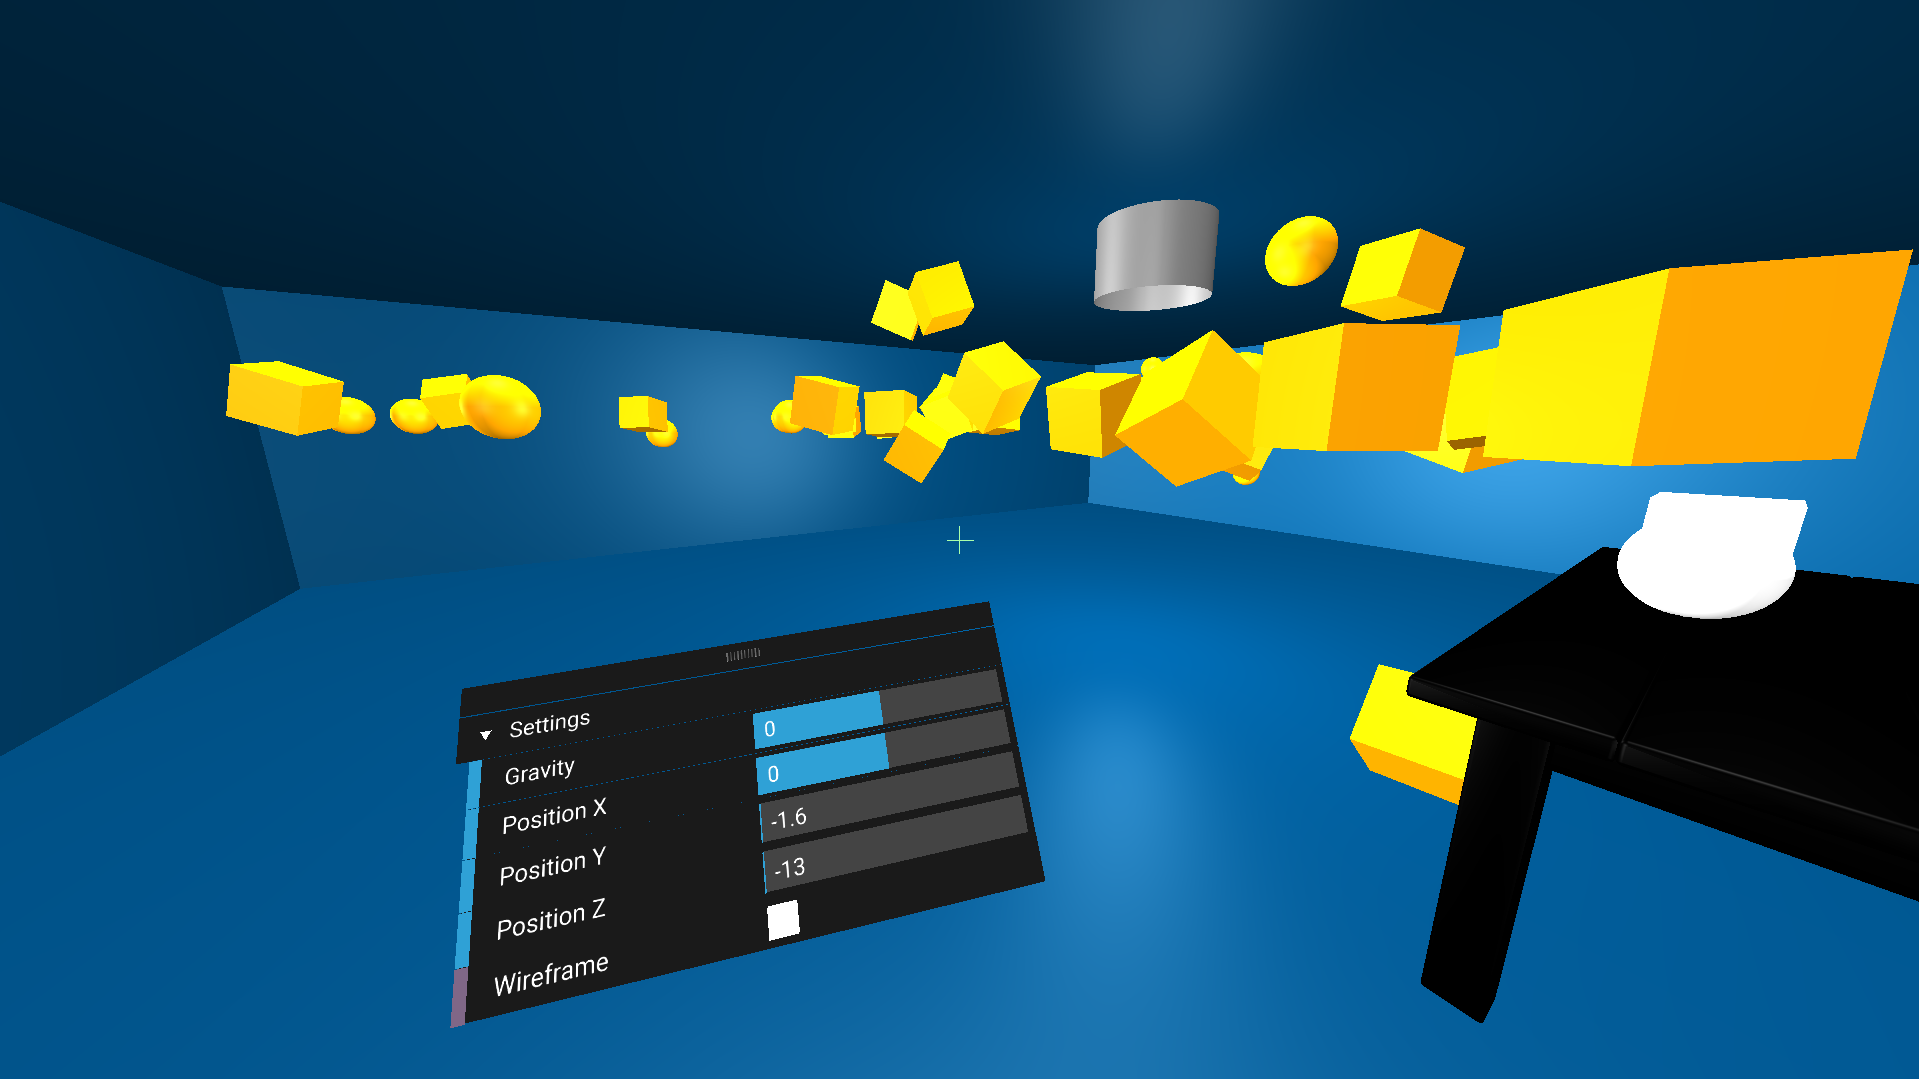
\includegraphics[width=\linewidth]{images/menu-gui-gravity.png}
    
\section{What we have left}
\subsection{Scene Environments}
Our current home room has a spinning cube in it from our initial testing.  We want to spiff it up with doors that navigate between each experiment.
\subsubsection{Asset acquisition}
We will be building or buying models to replace the placeholders that we have.
\subsubsection{3D Modeling}
Though some 3D modeling has already been done, more assets are needed for the experiences we plan to create in the coming weeks.
\subsection{Immersive Input}
\subsubsection{Single Controller}
We are currently working on implementing teleportation controls for both single and dual controller movement.
\subsubsection{Dual Controller}
Dual controller controls will use a teleportation control scheme similar to single controller controls.
\subsubsection{Gaze}
We want the app to work with basic "cardboard" virtual reality devices, which don't have a controller. The way we've decided to support these devices is to allow users to select objects by looking at them for an extended period of time. 
\subsection{Object Interaction}
We want a few generic object interactions like teleport and drag and drop, as well as specific interactions for each experiment.
\subsubsection{Raycast Selection}
Once each XR input device has been rendered into the scene, the user needs a way to interact with objects. A raycaster will be used to project a ray out the front of the rendered input device and used to calculate intersections with objects in the scene.
\subsubsection{Drag and Drop}
We need to support picking up objects and placing them down other places, so that users can reposition the objects and observe their interactions. 
\subsection{Physics Simulations}
\subsubsection{Planets Demo}
The planets demo has the core physics complete, but there are still several features we want to add. We want to add user interaction for pausing the simulation and viewing stats of a given planet. We also want to be able to add and remove planets from the system from within the simulation.
\subsubsection{Pendulum Mechanics}
The pendulum has yet to swing in a physically realistic way.  and needs to be able to be carried between tables.
\subsubsection{Core Kinematics}
So far, the experience is just a simple room with the basics of Cannon.js set up to create a ball that just falls to the floor. The goal is to create a sort of playground where the user can spawn in a variety of objects and be able to play around with them in a controllable environment. The user should eventually be able to change the laws of physics by manipulating gravity.
\subsubsection{Laser Refraction}
The refraction of light through certain materials is something we are interested in demonstrating on this site. Specifically, we want to provide an interactive laser refraction chamber to show how light behaves when it penetrates different materials. This experience has not been started yet. and requires assets, raycast input and light refraction equations.x
\subsection{Final Deployment to 01.org}
The last thing we need to do is deploy our site on 01.org, Intel's open source site. 

\section{Problems and Solutions}

% Changing implementation in chrome -> Watching when our devices update + looking at the Chrome change logs
% API changes
\subsection{API instability}
Since we are working with an API that is still in development, changes are to be expected. These changes create an instability in the API which has at times resulted in our code breaking. The only real solution to this is to stay up to date on the changes made to the API and implement any refactoring that needs to be done to our own code in response to these changes. Thankfully, the immersive web group keeps their git repositories and API reference page up to date with all changes. 
% Browser compatibility

% Issues differentiating between scroll to access descriptionary content -> Separate information page
\subsection{Scroll in the same page as VR experience}
One of the repeating problems we have been having is that scroll bars on the VR page cause our canvas to take up slightly more space than the page has, so there is a small amount of awkward scrolling when using the site. After struggling with this for a while, we have decided the best and most logical path forward is to move the content below our canvas, which introduces and links to each of the physics simulations, to a home page. This way, we can have our VR experience take up the entire page and we don't need to worry about scrolling at all. To us, this also seems like a more intuitive user experience.

% Deciding on sprint goals? -> pre-sprint research?

\subsection{Compatibility with other browsers}
Though we initially wrote of our site being compatible with a multitude of browsers, we quickly discovered that due to the nature of the WebXR API, this is simply not possible. Currently, the API is only compatible with the newest versions of Chrome Dev/Canary. Any user visiting the site from browsers other than these will not be able to get the full immersive XR experience. Fortunately, we have been working to add traditional controls to the site in the event that a user is unable to enter the immersive XR modes. For desktop computers without a connected HMD, mouse and keyboard controls have been added. Mobile devices have been given touch controls.

\end{document}